% Options for packages loaded elsewhere
\PassOptionsToPackage{unicode}{hyperref}
\PassOptionsToPackage{hyphens}{url}
%
\documentclass[
  ignorenonframetext,
]{beamer}
\usepackage{pgfpages}
\setbeamertemplate{caption}[numbered]
\setbeamertemplate{caption label separator}{: }
\setbeamercolor{caption name}{fg=normal text.fg}
\beamertemplatenavigationsymbolsempty
% Prevent slide breaks in the middle of a paragraph
\widowpenalties 1 10000
\raggedbottom
\setbeamertemplate{part page}{
  \centering
  \begin{beamercolorbox}[sep=16pt,center]{part title}
    \usebeamerfont{part title}\insertpart\par
  \end{beamercolorbox}
}
\setbeamertemplate{section page}{
  \centering
  \begin{beamercolorbox}[sep=12pt,center]{part title}
    \usebeamerfont{section title}\insertsection\par
  \end{beamercolorbox}
}
\setbeamertemplate{subsection page}{
  \centering
  \begin{beamercolorbox}[sep=8pt,center]{part title}
    \usebeamerfont{subsection title}\insertsubsection\par
  \end{beamercolorbox}
}
\AtBeginPart{
  \frame{\partpage}
}
\AtBeginSection{
  \ifbibliography
  \else
    \frame{\sectionpage}
  \fi
}
\AtBeginSubsection{
  \frame{\subsectionpage}
}
\usepackage{amsmath,amssymb}
\usepackage{iftex}
\ifPDFTeX
  \usepackage[T1]{fontenc}
  \usepackage[utf8]{inputenc}
  \usepackage{textcomp} % provide euro and other symbols
\else % if luatex or xetex
  \usepackage{unicode-math} % this also loads fontspec
  \defaultfontfeatures{Scale=MatchLowercase}
  \defaultfontfeatures[\rmfamily]{Ligatures=TeX,Scale=1}
\fi
\usepackage{lmodern}
\usetheme[]{Madrid}
\ifPDFTeX\else
  % xetex/luatex font selection
\fi
% Use upquote if available, for straight quotes in verbatim environments
\IfFileExists{upquote.sty}{\usepackage{upquote}}{}
\IfFileExists{microtype.sty}{% use microtype if available
  \usepackage[]{microtype}
  \UseMicrotypeSet[protrusion]{basicmath} % disable protrusion for tt fonts
}{}
\makeatletter
\@ifundefined{KOMAClassName}{% if non-KOMA class
  \IfFileExists{parskip.sty}{%
    \usepackage{parskip}
  }{% else
    \setlength{\parindent}{0pt}
    \setlength{\parskip}{6pt plus 2pt minus 1pt}}
}{% if KOMA class
  \KOMAoptions{parskip=half}}
\makeatother
\usepackage{xcolor}
\newif\ifbibliography
\usepackage{color}
\usepackage{fancyvrb}
\newcommand{\VerbBar}{|}
\newcommand{\VERB}{\Verb[commandchars=\\\{\}]}
\DefineVerbatimEnvironment{Highlighting}{Verbatim}{commandchars=\\\{\}}
% Add ',fontsize=\small' for more characters per line
\usepackage{framed}
\definecolor{shadecolor}{RGB}{248,248,248}
\newenvironment{Shaded}{\begin{snugshade}}{\end{snugshade}}
\newcommand{\AlertTok}[1]{\textcolor[rgb]{0.94,0.16,0.16}{#1}}
\newcommand{\AnnotationTok}[1]{\textcolor[rgb]{0.56,0.35,0.01}{\textbf{\textit{#1}}}}
\newcommand{\AttributeTok}[1]{\textcolor[rgb]{0.13,0.29,0.53}{#1}}
\newcommand{\BaseNTok}[1]{\textcolor[rgb]{0.00,0.00,0.81}{#1}}
\newcommand{\BuiltInTok}[1]{#1}
\newcommand{\CharTok}[1]{\textcolor[rgb]{0.31,0.60,0.02}{#1}}
\newcommand{\CommentTok}[1]{\textcolor[rgb]{0.56,0.35,0.01}{\textit{#1}}}
\newcommand{\CommentVarTok}[1]{\textcolor[rgb]{0.56,0.35,0.01}{\textbf{\textit{#1}}}}
\newcommand{\ConstantTok}[1]{\textcolor[rgb]{0.56,0.35,0.01}{#1}}
\newcommand{\ControlFlowTok}[1]{\textcolor[rgb]{0.13,0.29,0.53}{\textbf{#1}}}
\newcommand{\DataTypeTok}[1]{\textcolor[rgb]{0.13,0.29,0.53}{#1}}
\newcommand{\DecValTok}[1]{\textcolor[rgb]{0.00,0.00,0.81}{#1}}
\newcommand{\DocumentationTok}[1]{\textcolor[rgb]{0.56,0.35,0.01}{\textbf{\textit{#1}}}}
\newcommand{\ErrorTok}[1]{\textcolor[rgb]{0.64,0.00,0.00}{\textbf{#1}}}
\newcommand{\ExtensionTok}[1]{#1}
\newcommand{\FloatTok}[1]{\textcolor[rgb]{0.00,0.00,0.81}{#1}}
\newcommand{\FunctionTok}[1]{\textcolor[rgb]{0.13,0.29,0.53}{\textbf{#1}}}
\newcommand{\ImportTok}[1]{#1}
\newcommand{\InformationTok}[1]{\textcolor[rgb]{0.56,0.35,0.01}{\textbf{\textit{#1}}}}
\newcommand{\KeywordTok}[1]{\textcolor[rgb]{0.13,0.29,0.53}{\textbf{#1}}}
\newcommand{\NormalTok}[1]{#1}
\newcommand{\OperatorTok}[1]{\textcolor[rgb]{0.81,0.36,0.00}{\textbf{#1}}}
\newcommand{\OtherTok}[1]{\textcolor[rgb]{0.56,0.35,0.01}{#1}}
\newcommand{\PreprocessorTok}[1]{\textcolor[rgb]{0.56,0.35,0.01}{\textit{#1}}}
\newcommand{\RegionMarkerTok}[1]{#1}
\newcommand{\SpecialCharTok}[1]{\textcolor[rgb]{0.81,0.36,0.00}{\textbf{#1}}}
\newcommand{\SpecialStringTok}[1]{\textcolor[rgb]{0.31,0.60,0.02}{#1}}
\newcommand{\StringTok}[1]{\textcolor[rgb]{0.31,0.60,0.02}{#1}}
\newcommand{\VariableTok}[1]{\textcolor[rgb]{0.00,0.00,0.00}{#1}}
\newcommand{\VerbatimStringTok}[1]{\textcolor[rgb]{0.31,0.60,0.02}{#1}}
\newcommand{\WarningTok}[1]{\textcolor[rgb]{0.56,0.35,0.01}{\textbf{\textit{#1}}}}
\usepackage{graphicx}
\makeatletter
\def\maxwidth{\ifdim\Gin@nat@width>\linewidth\linewidth\else\Gin@nat@width\fi}
\def\maxheight{\ifdim\Gin@nat@height>\textheight\textheight\else\Gin@nat@height\fi}
\makeatother
% Scale images if necessary, so that they will not overflow the page
% margins by default, and it is still possible to overwrite the defaults
% using explicit options in \includegraphics[width, height, ...]{}
\setkeys{Gin}{width=\maxwidth,height=\maxheight,keepaspectratio}
% Set default figure placement to htbp
\makeatletter
\def\fps@figure{htbp}
\makeatother
\setlength{\emergencystretch}{3em} % prevent overfull lines
\providecommand{\tightlist}{%
  \setlength{\itemsep}{0pt}\setlength{\parskip}{0pt}}
\setcounter{secnumdepth}{-\maxdimen} % remove section numbering
\logo{
\includegraphics[height=1cm,width=3cm]{logo.png}}
\usetheme{Madrid}
\usefonttheme{serif}
\setbeamertemplate{navigation symbols}{}
\usepackage{lmodern}  % for bold teletype font
\usepackage{amsmath}  % for \hookrightarrow
\usepackage{xcolor}   % for \textcolor


\ifLuaTeX
  \usepackage{selnolig}  % disable illegal ligatures
\fi
\usepackage{bookmark}
\IfFileExists{xurl.sty}{\usepackage{xurl}}{} % add URL line breaks if available
\urlstyle{same}
\hypersetup{
  pdftitle={Leksioni 12},
  pdfauthor={Endri Raco},
  hidelinks,
  pdfcreator={LaTeX via pandoc}}

\title{Leksioni 12}
\author{Endri Raco}
\date{03 July, 2024}

\begin{document}
\frame{\titlepage}

\begin{frame}[allowframebreaks]
  \tableofcontents[hideallsubsections]
\end{frame}
\section{Hyrje në SQL}\label{hyrje-nuxeb-sql}

\begin{frame}{Hyrje në SQL}
\phantomsection\label{hyrje-nuxeb-sql-1}
SQL është një gjuhë standarde për aksesin dhe manipulimin e bazave të të
dhënave.
\end{frame}

\begin{frame}{Çfarë është SQL?}
\phantomsection\label{uxe7faruxeb-uxebshtuxeb-sql}
\begin{itemize}
\item
  SQL qëndron për Structured Query Language
\item
  SQL ju lejon të aksesoni dhe manipuloni bazat e të dhënave
\end{itemize}
\end{frame}

\begin{frame}{Çfarë mund të bëjë SQL?}
\phantomsection\label{uxe7faruxeb-mund-tuxeb-buxebjuxeb-sql}
\begin{itemize}
\item
  SQL mund të ekzekutojë pyetje \textbf{query} në një baze të dhënash
\item
  SQL mund të marrë të dhëna nga një bazë të dhënash
\item
  SQL mund të fusë të dhëna në një bazë të dhënash
\end{itemize}
\end{frame}

\begin{frame}{Çfarë mund të bëjë SQL?}
\phantomsection\label{uxe7faruxeb-mund-tuxeb-buxebjuxeb-sql-1}
\begin{itemize}
\item
  SQL mund të përditësojë të dhënat në një bazë të dhënash
\item
  SQL mund të fshijë të dhënat nga një bazë të dhënash
\item
  SQL mund të krijojë baza të reja të dhënash
\end{itemize}
\end{frame}

\begin{frame}{Çfarë mund të bëjë SQL?}
\phantomsection\label{uxe7faruxeb-mund-tuxeb-buxebjuxeb-sql-2}
\begin{itemize}
\item
  SQL mund të krijojë tabela të reja në një bazë të dhënash
\item
  SQL mund të krijojë procedura të ruajtura në një bazë të dhënash
\end{itemize}

SQL mund të krijojë pamje \textbf{views} në një bazë të dhënash
\end{frame}

\begin{frame}{Çfarë mund të bëjë SQL?}
\phantomsection\label{uxe7faruxeb-mund-tuxeb-buxebjuxeb-sql-3}
\begin{itemize}
\tightlist
\item
  Megjithëse SQL është një standard ANSI/ISO, ekzistojnë versione të
  ndryshme të gjuhës SQL.
\end{itemize}
\end{frame}

\begin{frame}{Çfarë mund të bëjë SQL?}
\phantomsection\label{uxe7faruxeb-mund-tuxeb-buxebjuxeb-sql-4}
Sidoqoftë, për të qenë në përputhje me standardin ANSI, të gjitha ato
mbështesin të paktën komandat kryesore (siç janë SELECT, UPDATE, DELETE,
INSERT, WHERE) në një mënyrë të ngjashme.
\end{frame}

\begin{frame}{RDBMS}
\phantomsection\label{rdbms}
\begin{itemize}
\item
  RDBMS do të thotë Sistemi i Menaxhimit të Bazave të të Dhënave
  Relacionale.
\item
  RDBMS është baza për SQL dhe për të gjitha sistemet moderne të bazës
  së të dhënave si MS SQL Server, IBM DB2, Oracle, MySQL dhe Microsoft
  Access.
\end{itemize}
\end{frame}

\begin{frame}{RDBMS}
\phantomsection\label{rdbms-1}
\begin{itemize}
\tightlist
\item
  Të dhënat në RDBMS ruhen në objektet e bazës së të dhënave të quajtura
  tabela.
\end{itemize}
\end{frame}

\begin{frame}[fragile]{Fillojmë me një tabelë}
\phantomsection\label{fillojmuxeb-me-njuxeb-tabeluxeb}
\AddToHookNext{env/Highlighting/begin}{\tiny}

\begin{Shaded}
\begin{Highlighting}[]
\CommentTok{{-}{-} Krijo tabelën Klientë}
\KeywordTok{CREATE} \KeywordTok{TABLE}\NormalTok{ Klientë (}
\NormalTok{  idKlienti }\DataTypeTok{int} \KeywordTok{PRIMARY} \KeywordTok{KEY}\NormalTok{ IDENTITY(}\DecValTok{1}\NormalTok{,}\DecValTok{1}\NormalTok{),}
\NormalTok{  emri }\DataTypeTok{varchar}\NormalTok{(}\DecValTok{50}\NormalTok{) }\KeywordTok{NOT} \KeywordTok{NULL}\NormalTok{,}
\NormalTok{  mbiemri }\DataTypeTok{varchar}\NormalTok{(}\DecValTok{50}\NormalTok{) }\KeywordTok{NOT} \KeywordTok{NULL}\NormalTok{,}
\NormalTok{  email }\DataTypeTok{varchar}\NormalTok{(}\DecValTok{100}\NormalTok{) }\KeywordTok{NOT} \KeywordTok{NULL} \KeywordTok{UNIQUE}\NormalTok{,}
\NormalTok{  telefoni }\DataTypeTok{varchar}\NormalTok{(}\DecValTok{20}\NormalTok{),}
\NormalTok{  adresa }\DataTypeTok{varchar}\NormalTok{(}\DecValTok{255}\NormalTok{),}
\NormalTok{  qyteti }\DataTypeTok{varchar}\NormalTok{(}\DecValTok{50}\NormalTok{),}
\NormalTok{  shteti }\DataTypeTok{varchar}\NormalTok{(}\DecValTok{50}\NormalTok{),}
\NormalTok{  kodi\_postar }\DataTypeTok{varchar}\NormalTok{(}\DecValTok{10}\NormalTok{),}
\NormalTok{  data\_regjistrimit }\DataTypeTok{DATE} \KeywordTok{DEFAULT}\NormalTok{ GETDATE()}
\NormalTok{);}
\end{Highlighting}
\end{Shaded}
\end{frame}

\begin{frame}[fragile]{Fillojmë me një tabelë}
\phantomsection\label{fillojmuxeb-me-njuxeb-tabeluxeb-1}
\AddToHookNext{env/Highlighting/begin}{\tiny}

\begin{Shaded}
\begin{Highlighting}[]
\CommentTok{{-}{-} Mbush tabelën Klientë me të dhëna shembull}
\KeywordTok{INSERT} \KeywordTok{INTO}\NormalTok{ Klientë (emri, mbiemri, email, telefoni, adresa, qyteti, shteti, kodi\_postar)}
\KeywordTok{VALUES}\NormalTok{ (}\StringTok{\textquotesingle{}Ana\textquotesingle{}}\NormalTok{, }\StringTok{\textquotesingle{}Hoxha\textquotesingle{}}\NormalTok{, }\StringTok{\textquotesingle{}ana.hoxha@example.com\textquotesingle{}}\NormalTok{, }\StringTok{\textquotesingle{}0681234567\textquotesingle{}}\NormalTok{, }\StringTok{\textquotesingle{}Rruga e Dibrës 12\textquotesingle{}}\NormalTok{, }\StringTok{\textquotesingle{}Tiranë\textquotesingle{}}\NormalTok{, }\StringTok{\textquotesingle{}Shqipëri\textquotesingle{}}\NormalTok{, }\StringTok{\textquotesingle{}1001\textquotesingle{}}\NormalTok{);}

\CommentTok{{-}{-} Mbush tabelën Klientë me të dhëna shembull}
\KeywordTok{INSERT} \KeywordTok{INTO}\NormalTok{ Klientë (emri, mbiemri, email, telefoni, adresa, qyteti, shteti, kodi\_postar)}
\KeywordTok{VALUES}\NormalTok{ (}\StringTok{\textquotesingle{}Maria\textquotesingle{}}\NormalTok{, }\StringTok{\textquotesingle{}Anders\textquotesingle{}}\NormalTok{, }\StringTok{\textquotesingle{}maria.anders@alfredsfutterkiste.com\textquotesingle{}}\NormalTok{, }\StringTok{\textquotesingle{}0123456789\textquotesingle{}}\NormalTok{, }\StringTok{\textquotesingle{}Obere Str. 57\textquotesingle{}}\NormalTok{, }\StringTok{\textquotesingle{}Berlin\textquotesingle{}}\NormalTok{, }\StringTok{\textquotesingle{}Germany\textquotesingle{}}\NormalTok{, }\StringTok{\textquotesingle{}12209\textquotesingle{}}\NormalTok{);}

\KeywordTok{INSERT} \KeywordTok{INTO}\NormalTok{ Klientë (emri, mbiemri, email, telefoni, adresa, qyteti, shteti, kodi\_postar)}
\KeywordTok{VALUES}\NormalTok{ (}\StringTok{\textquotesingle{}Ana\textquotesingle{}}\NormalTok{, }\StringTok{\textquotesingle{}Trujillo\textquotesingle{}}\NormalTok{, }\StringTok{\textquotesingle{}ana.trujillo@emparedadosyhelados.com\textquotesingle{}}\NormalTok{, }\StringTok{\textquotesingle{}9876543210\textquotesingle{}}\NormalTok{, }\StringTok{\textquotesingle{}Avda. de la Constitución 2222\textquotesingle{}}\NormalTok{, }\StringTok{\textquotesingle{}México D.F.\textquotesingle{}}\NormalTok{, }\StringTok{\textquotesingle{}Mexico\textquotesingle{}}\NormalTok{, }\StringTok{\textquotesingle{}05021\textquotesingle{}}\NormalTok{);}

\KeywordTok{INSERT} \KeywordTok{INTO}\NormalTok{ Klientë (emri, mbiemri, email, telefoni, adresa, qyteti, shteti, kodi\_postar)}
\KeywordTok{VALUES}\NormalTok{ (}\StringTok{\textquotesingle{}Antonio\textquotesingle{}}\NormalTok{, }\StringTok{\textquotesingle{}Moreno\textquotesingle{}}\NormalTok{, }\StringTok{\textquotesingle{}antonio.moreno@taqueria.com\textquotesingle{}}\NormalTok{, }\StringTok{\textquotesingle{}1234567890\textquotesingle{}}\NormalTok{, }\StringTok{\textquotesingle{}Mataderos 2312\textquotesingle{}}\NormalTok{, }\StringTok{\textquotesingle{}México D.F.\textquotesingle{}}\NormalTok{, }\StringTok{\textquotesingle{}Mexico\textquotesingle{}}\NormalTok{, }\StringTok{\textquotesingle{}05023\textquotesingle{}}\NormalTok{);}

\KeywordTok{INSERT} \KeywordTok{INTO}\NormalTok{ Klientë (emri, mbiemri, email, telefoni, adresa, qyteti, shteti, kodi\_postar)}
\KeywordTok{VALUES}\NormalTok{ (}\StringTok{\textquotesingle{}Thomas\textquotesingle{}}\NormalTok{, }\StringTok{\textquotesingle{}Hardy\textquotesingle{}}\NormalTok{, }\StringTok{\textquotesingle{}thomas.hardy@aroundthehorn.com\textquotesingle{}}\NormalTok{, }\StringTok{\textquotesingle{}2345678901\textquotesingle{}}\NormalTok{, }\StringTok{\textquotesingle{}120 Hanover Sq.\textquotesingle{}}\NormalTok{, }\StringTok{\textquotesingle{}London\textquotesingle{}}\NormalTok{, }\StringTok{\textquotesingle{}UK\textquotesingle{}}\NormalTok{, }\StringTok{\textquotesingle{}WA1 1DP\textquotesingle{}}\NormalTok{);}

\KeywordTok{INSERT} \KeywordTok{INTO}\NormalTok{ Klientë (emri, mbiemri, email, telefoni, adresa, qyteti, shteti, kodi\_postar)}
\KeywordTok{VALUES}\NormalTok{ (}\StringTok{\textquotesingle{}Christina\textquotesingle{}}\NormalTok{, }\StringTok{\textquotesingle{}Berglund\textquotesingle{}}\NormalTok{, }\StringTok{\textquotesingle{}christina.berglund@berglundssnabbkop.com\textquotesingle{}}\NormalTok{, }\StringTok{\textquotesingle{}3456789012\textquotesingle{}}\NormalTok{, }\StringTok{\textquotesingle{}Berguvsvägen 8\textquotesingle{}}\NormalTok{, }\StringTok{\textquotesingle{}Luleå\textquotesingle{}}\NormalTok{, }\StringTok{\textquotesingle{}Sweden\textquotesingle{}}\NormalTok{, }\StringTok{\textquotesingle{}S{-}958 22\textquotesingle{}}\NormalTok{);}
\end{Highlighting}
\end{Shaded}
\end{frame}

\begin{frame}[fragile]{Shikoni tabelën ``Klientë''}
\phantomsection\label{shikoni-tabeluxebn-klientuxeb}
\begin{Shaded}
\begin{Highlighting}[]
\KeywordTok{SELECT} \OperatorTok{*} \KeywordTok{FROM}\NormalTok{ Klientë;}
\end{Highlighting}
\end{Shaded}
\end{frame}

\begin{frame}{Shikoni tabelën ``Klientë''}
\phantomsection\label{shikoni-tabeluxebn-klientuxeb-1}
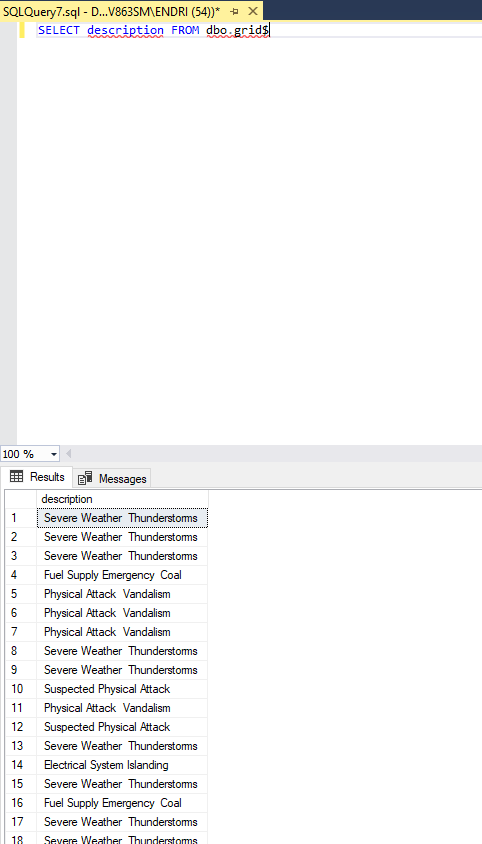
\includegraphics{./Figs/query1.png}
\end{frame}

\begin{frame}{Struktura e Databazave}
\phantomsection\label{struktura-e-databazave}
\begin{itemize}
\item
  Çdo tabelë ndahet në entitete më të vogla të quajtura fusha.
\item
  Fushat në tabelën e klientëve përbëhen nga ID-ja e klientit, emri i
  klientit, emri i kontaktit, adresa, qyteti, kodi postar dhe shteti.
\end{itemize}
\end{frame}

\begin{frame}{Struktura e Databazave}
\phantomsection\label{struktura-e-databazave-1}
\begin{itemize}
\tightlist
\item
  Një fushë është një kolonë në një tabelë që është krijuar për të
  mbajtur informacion specifik për çdo regjistrim në tabelë.
\end{itemize}
\end{frame}

\begin{frame}{Struktura e Databazave}
\phantomsection\label{struktura-e-databazave-2}
\begin{itemize}
\item
  Një rekord, i quajtur gjithashtu një rresht, është çdo hyrje
  individuale që ekziston në një tabelë.
\item
  Për shembull, ka 5 regjistrime në tabelën e mësipërme të klientëve.
\end{itemize}
\end{frame}

\begin{frame}{Struktura e Databazave}
\phantomsection\label{struktura-e-databazave-3}
\begin{itemize}
\item
  Një rekord është një entitet horizontal në një tabelë.
\item
  Një kolonë është një entitet vertikal në një tabelë që përmban të
  gjithë informacionin e lidhur me një fushë specifike në një tabelë.
\end{itemize}
\end{frame}

\begin{frame}{Deklarata SELECT}
\phantomsection\label{deklarata-select}
Deklarata SELECT përdoret për të zgjedhur të dhënat nga një bazë të
dhënash.
\end{frame}

\begin{frame}[fragile]{Shembull : Ktheni të dhënat nga tabela e
klientëve}
\phantomsection\label{shembull-ktheni-tuxeb-dhuxebnat-nga-tabela-e-klientuxebve}
\begin{Shaded}
\begin{Highlighting}[]
\KeywordTok{SELECT}\NormalTok{ emri, qyteti }\KeywordTok{FROM}\NormalTok{ Klientë;}
\end{Highlighting}
\end{Shaded}
\end{frame}

\begin{frame}{Shembull : Ktheni të dhënat nga tabela e klientëve}
\phantomsection\label{shembull-ktheni-tuxeb-dhuxebnat-nga-tabela-e-klientuxebve-1}
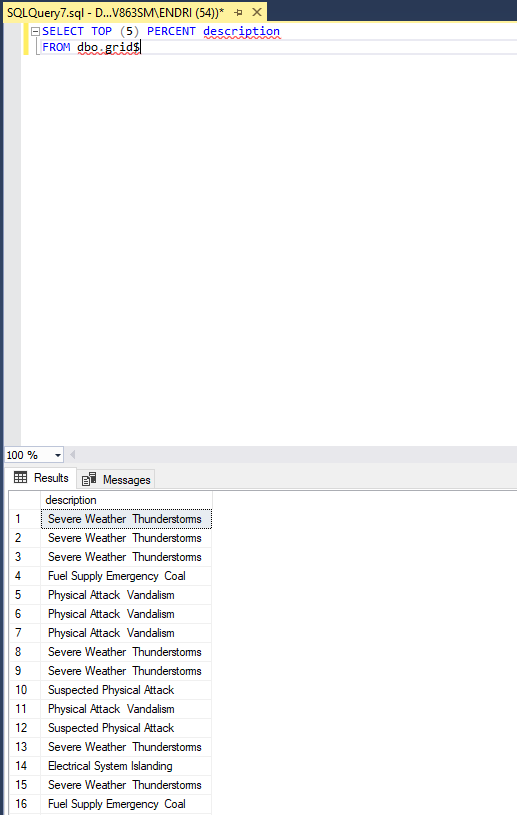
\includegraphics{./Figs/query2.png}
\end{frame}

\begin{frame}[fragile]{Sintaksë}
\phantomsection\label{sintaksuxeb}
\begin{Shaded}
\begin{Highlighting}[]
\KeywordTok{SELECT}\NormalTok{ kolonën }\DecValTok{1}\NormalTok{, kolonën }\DecValTok{2}\NormalTok{, }\OperatorTok{..}\NormalTok{.}
\KeywordTok{FROM}\NormalTok{ emri\_tabelës;}
\end{Highlighting}
\end{Shaded}

Këtu, kolona 1, kolona 2, \ldots{} janë emrat e fushave të tabelës nga
të cilat dëshironi të zgjidhni të dhënat.

Emri\_tabela përfaqëson emrin e tabelës nga e cila dëshironi të zgjidhni
të dhënat.
\end{frame}

\begin{frame}{Zgjidhni TË GJITHA kolonat}
\phantomsection\label{zgjidhni-tuxeb-gjitha-kolonat}
Nëse dëshironi të ktheni të gjitha kolonat, pa specifikuar emrin e çdo
kolone, mund të përdorni sintaksën SELECT *:
\end{frame}

\begin{frame}[fragile]{Zgjidhni TË GJITHA kolonat}
\phantomsection\label{zgjidhni-tuxeb-gjitha-kolonat-1}
Ktheni të gjitha kolonat nga tabela Klientë:

\begin{Shaded}
\begin{Highlighting}[]
\KeywordTok{SELECT} \OperatorTok{*}\NormalTok{ NGA Klientë}
\end{Highlighting}
\end{Shaded}
\end{frame}

\begin{frame}{Zgjidhni TË GJITHA kolonat}
\phantomsection\label{zgjidhni-tuxeb-gjitha-kolonat-2}
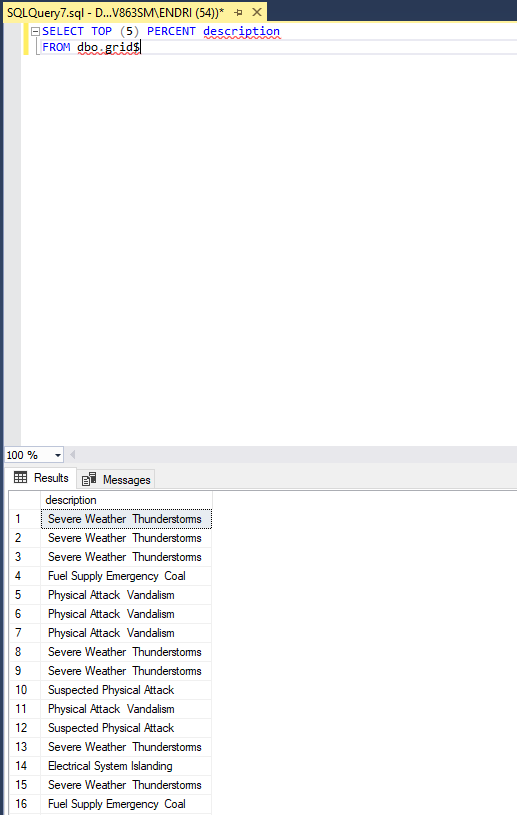
\includegraphics{./Figs/query2.png}
\end{frame}

\begin{frame}{Deklarata SELECT DISTINCT}
\phantomsection\label{deklarata-select-distinct}
\begin{itemize}
\tightlist
\item
  Deklarata SELECT DISTINCT përdoret për të kthyer vetëm vlera të
  dallueshme (të ndryshme).
\end{itemize}
\end{frame}

\begin{frame}[fragile]{Zgjidhni të gjitha shtetet e ndryshme}
\phantomsection\label{zgjidhni-tuxeb-gjitha-shtetet-e-ndryshme}
Zgjidhni të gjitha shtetet e ndryshme nga tabela ``Klientë''

\begin{Shaded}
\begin{Highlighting}[]
\KeywordTok{SELECT} \KeywordTok{DISTINCT}\NormalTok{ shteti }\KeywordTok{FROM}\NormalTok{  Klientë}
\end{Highlighting}
\end{Shaded}
\end{frame}

\begin{frame}{Zgjidhni të gjitha shtetet e ndryshme}
\phantomsection\label{zgjidhni-tuxeb-gjitha-shtetet-e-ndryshme-1}
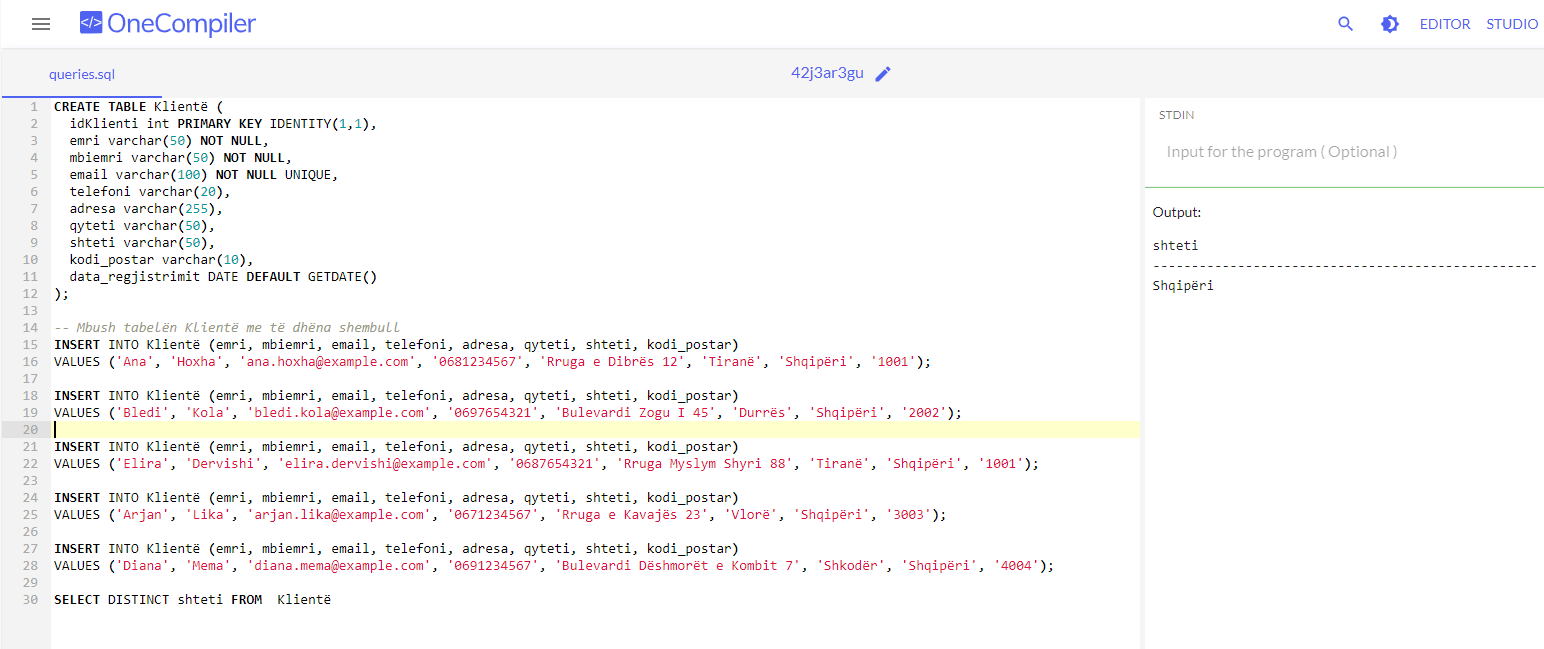
\includegraphics{./Figs/query3.png}
\end{frame}

\begin{frame}{Zgjidhni të gjitha shtetet e ndryshme}
\phantomsection\label{zgjidhni-tuxeb-gjitha-shtetet-e-ndryshme-2}
\begin{itemize}
\tightlist
\item
  Brenda një tabele, një kolonë shpesh përmban shumë vlera të kopjuara;
  dhe ndonjëherë ju dëshironi vetëm të listoni vlerat e ndryshme (të
  dallueshme).
\end{itemize}
\end{frame}

\begin{frame}{Zgjidhni pa DISTINCT}
\phantomsection\label{zgjidhni-pa-distinct}
\begin{itemize}
\tightlist
\item
  Nëse e hiqni fjalën kyçe DISTINCT, deklarata SQL kthen vlerën
  ``shteti'' nga të gjitha të dhënat e tabelës ``Klientë'':
\end{itemize}
\end{frame}

\begin{frame}[fragile]{Zgjidhni të gjitha shtetet e ndryshme}
\phantomsection\label{zgjidhni-tuxeb-gjitha-shtetet-e-ndryshme-3}
Zgjidhni të gjitha shtetet e ndryshme nga tabela ``Klientë''

\begin{Shaded}
\begin{Highlighting}[]
\KeywordTok{SELECT}\NormalTok{ shteti }\KeywordTok{FROM}\NormalTok{  Klientë}
\end{Highlighting}
\end{Shaded}
\end{frame}

\begin{frame}{Zgjidhni të gjitha shtetet e ndryshme}
\phantomsection\label{zgjidhni-tuxeb-gjitha-shtetet-e-ndryshme-4}
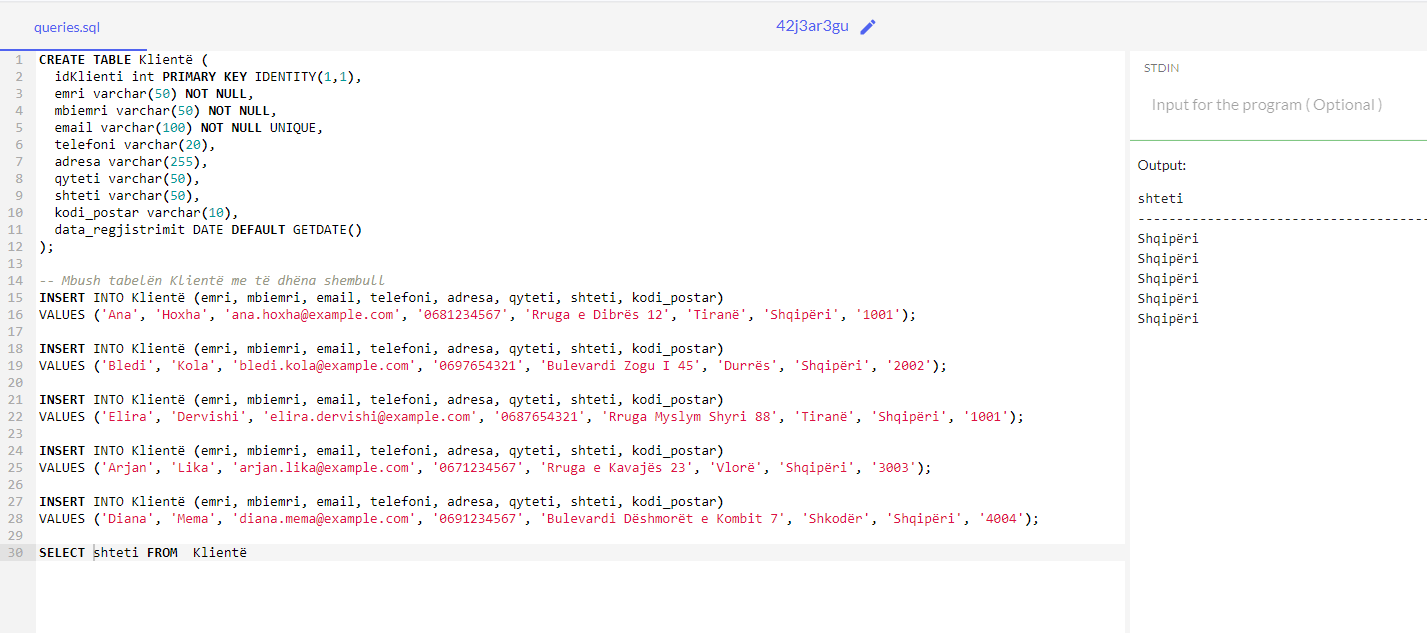
\includegraphics{./Figs/query4.png}
\end{frame}

\begin{frame}{Numërimi me DISTINCT}
\phantomsection\label{numuxebrimi-me-distinct}
\begin{itemize}
\tightlist
\item
  Duke përdorur fjalën kyçe DISTINCT në një funksion të quajtur COUNT,
  ne mund të kthejmë numrin e vendeve të ndryshme.
\end{itemize}
\end{frame}

\begin{frame}[fragile]{Shembull}
\phantomsection\label{shembull}
\begin{Shaded}
\begin{Highlighting}[]
\KeywordTok{SELECT} \FunctionTok{COUNT}\NormalTok{(}\KeywordTok{DISTINCT}\NormalTok{ shteti) }\KeywordTok{FROM}\NormalTok{ Klientë}
\end{Highlighting}
\end{Shaded}
\end{frame}

\begin{frame}{Zgjidhni të gjitha shtetet e ndryshme}
\phantomsection\label{zgjidhni-tuxeb-gjitha-shtetet-e-ndryshme-5}
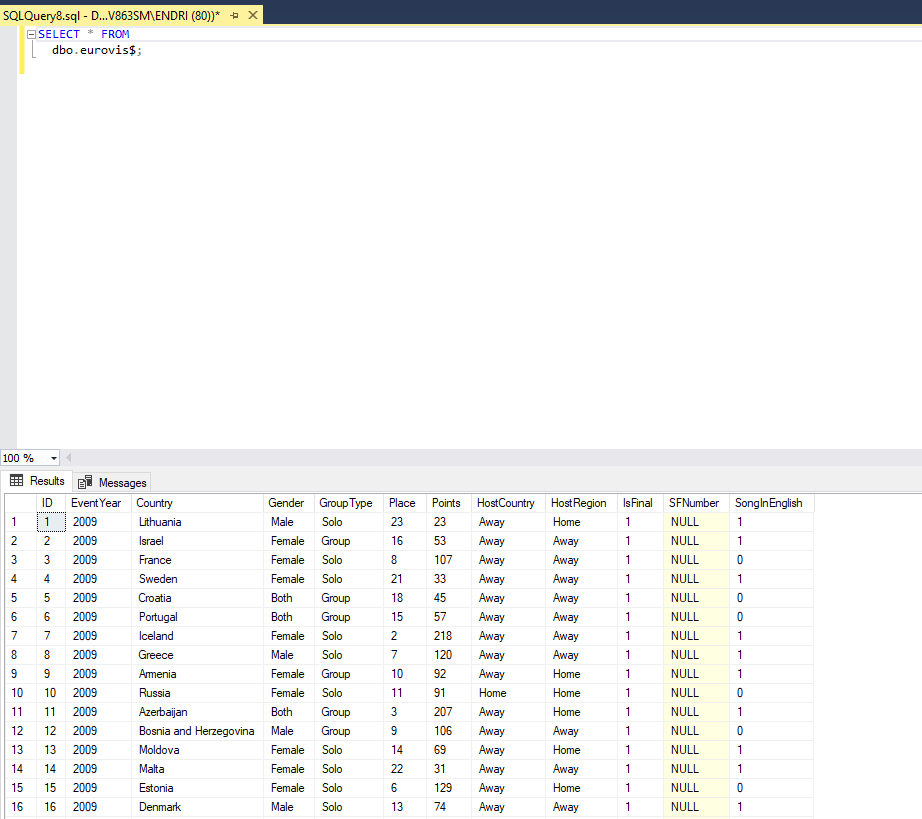
\includegraphics{./Figs/query5.png}
\end{frame}

\begin{frame}{Deklarata WHERE}
\phantomsection\label{deklarata-where}
\begin{itemize}
\item
  Klauzola WHERE përdoret për të filtruar të dhënat.
\item
  Përdoret për të nxjerrë vetëm ato rekorde që plotësojnë një kusht të
  caktuar.
\end{itemize}
\end{frame}

\begin{frame}[fragile]{Shembull}
\phantomsection\label{shembull-1}
\begin{Shaded}
\begin{Highlighting}[]
\KeywordTok{SELECT} \OperatorTok{*} \KeywordTok{FROM}\NormalTok{ Klientë}
\KeywordTok{WHERE}\NormalTok{ shteti}\OperatorTok{=}\StringTok{\textquotesingle{}Mexico\textquotesingle{}}
\end{Highlighting}
\end{Shaded}
\end{frame}

\begin{frame}{Shembull}
\phantomsection\label{shembull-2}
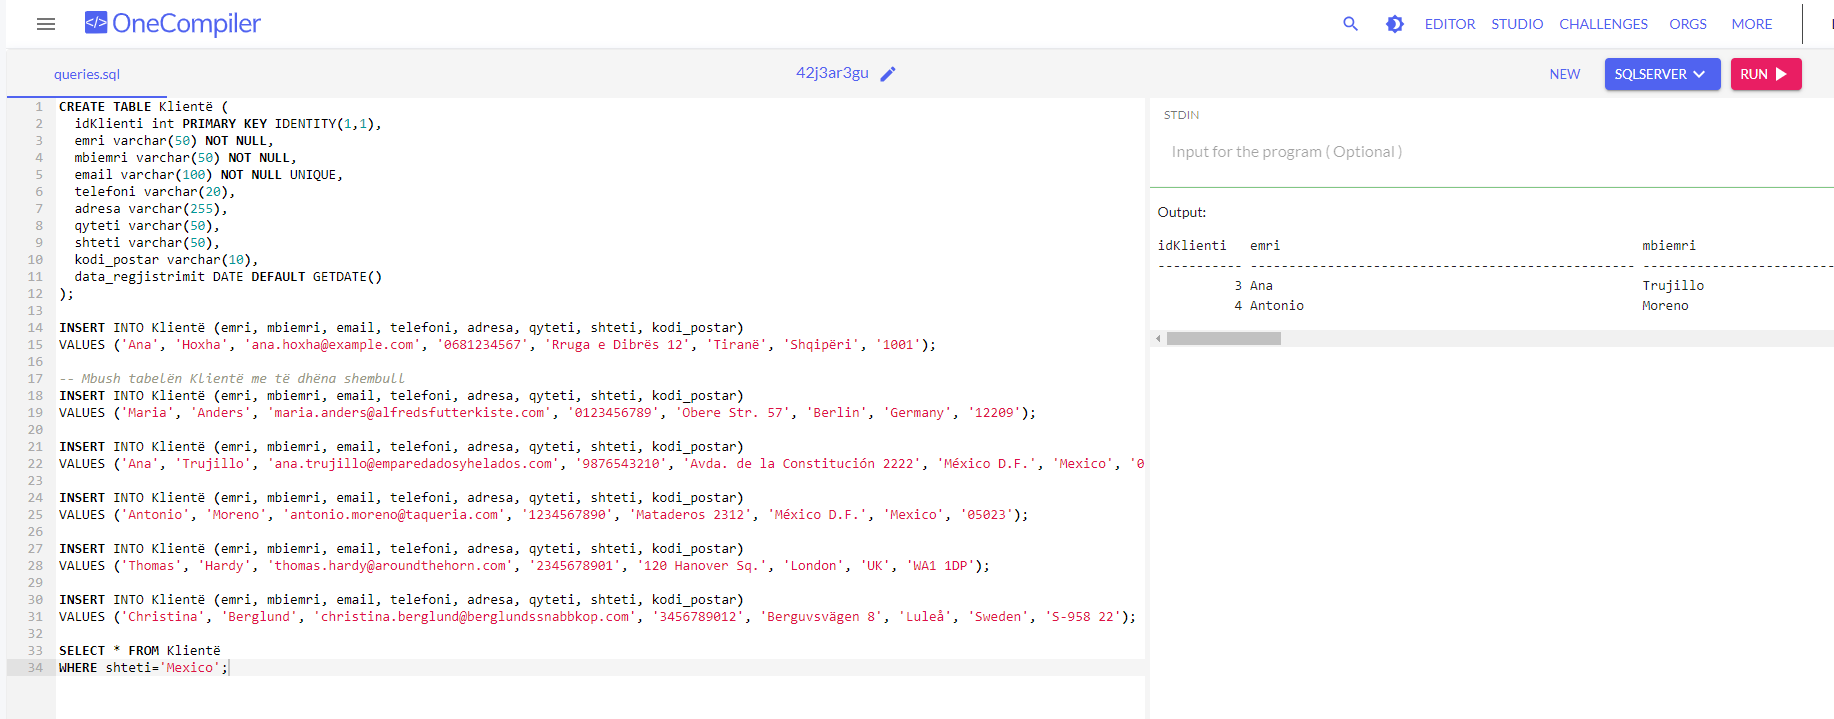
\includegraphics{./Figs/query6.png}
\end{frame}

\begin{frame}{Fushat tekst kundrejt fushave numerike}
\phantomsection\label{fushat-tekst-kundrejt-fushave-numerike}
\begin{itemize}
\item
  SQL kërkon thonjëza të vetme rreth vlerave të tekstit (shumica e
  sistemeve të bazës së të dhënave do të lejojnë gjithashtu thonjëza të
  dyfishta).
\item
  Sidoqoftë, fushat numerike nuk duhet të mbyllen në thonjëza:
\end{itemize}
\end{frame}

\begin{frame}[fragile]{Shembull}
\phantomsection\label{shembull-3}
\begin{Shaded}
\begin{Highlighting}[]
\KeywordTok{SELECT} \OperatorTok{*} \KeywordTok{FROM}\NormalTok{ Klientë}
\KeywordTok{WHERE}\NormalTok{ idKlienti }\OperatorTok{=}\DecValTok{1}
\end{Highlighting}
\end{Shaded}
\end{frame}

\begin{frame}{Shembull}
\phantomsection\label{shembull-4}
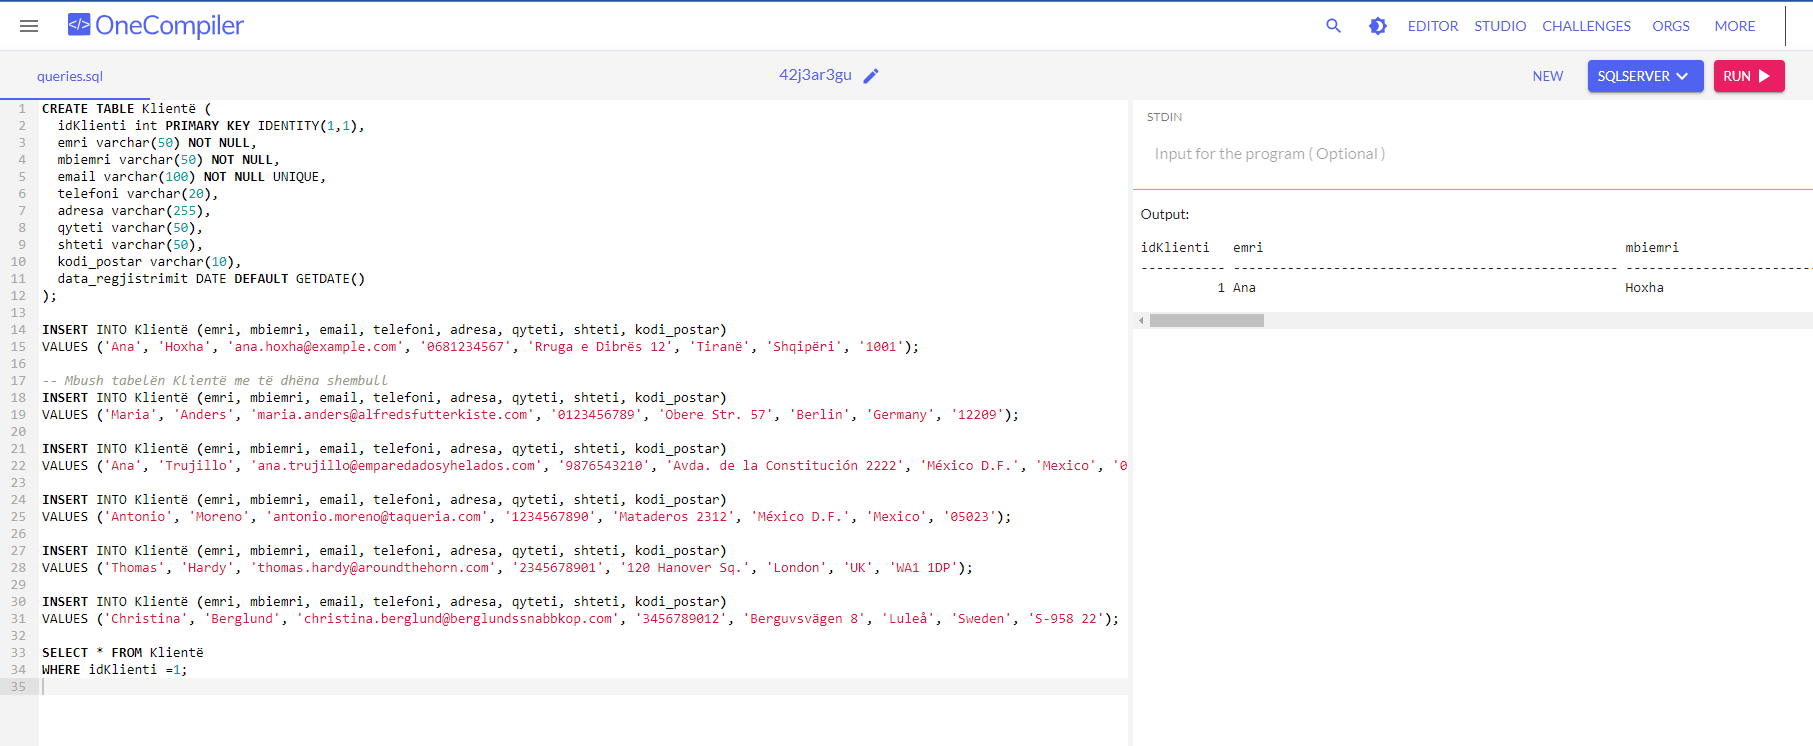
\includegraphics{./Figs/query7.png}
\end{frame}

\begin{frame}{Operatorët IN klauzolën WHERE}
\phantomsection\label{operatoruxebt-in-klauzoluxebn-where}
\begin{itemize}
\tightlist
\item
  Ju mund të përdorni operatorë të tjerë përveç operatorit \textbf{=}
  për të filtruar kërkimin.
\end{itemize}
\end{frame}

\begin{frame}{Shembull}
\phantomsection\label{shembull-5}
Zgjidhni të gjithë klientët me një ID klienti më të madh se 80:
\end{frame}

\begin{frame}[fragile]{Shembull}
\phantomsection\label{shembull-6}
\begin{Shaded}
\begin{Highlighting}[]
\KeywordTok{SELECT} \OperatorTok{*} \KeywordTok{FROM}\NormalTok{ Klientë}
\KeywordTok{WHERE}\NormalTok{ idKlienti }\OperatorTok{\textgreater{}} \DecValTok{80}
\end{Highlighting}
\end{Shaded}
\end{frame}

\begin{frame}{Shembull}
\phantomsection\label{shembull-7}
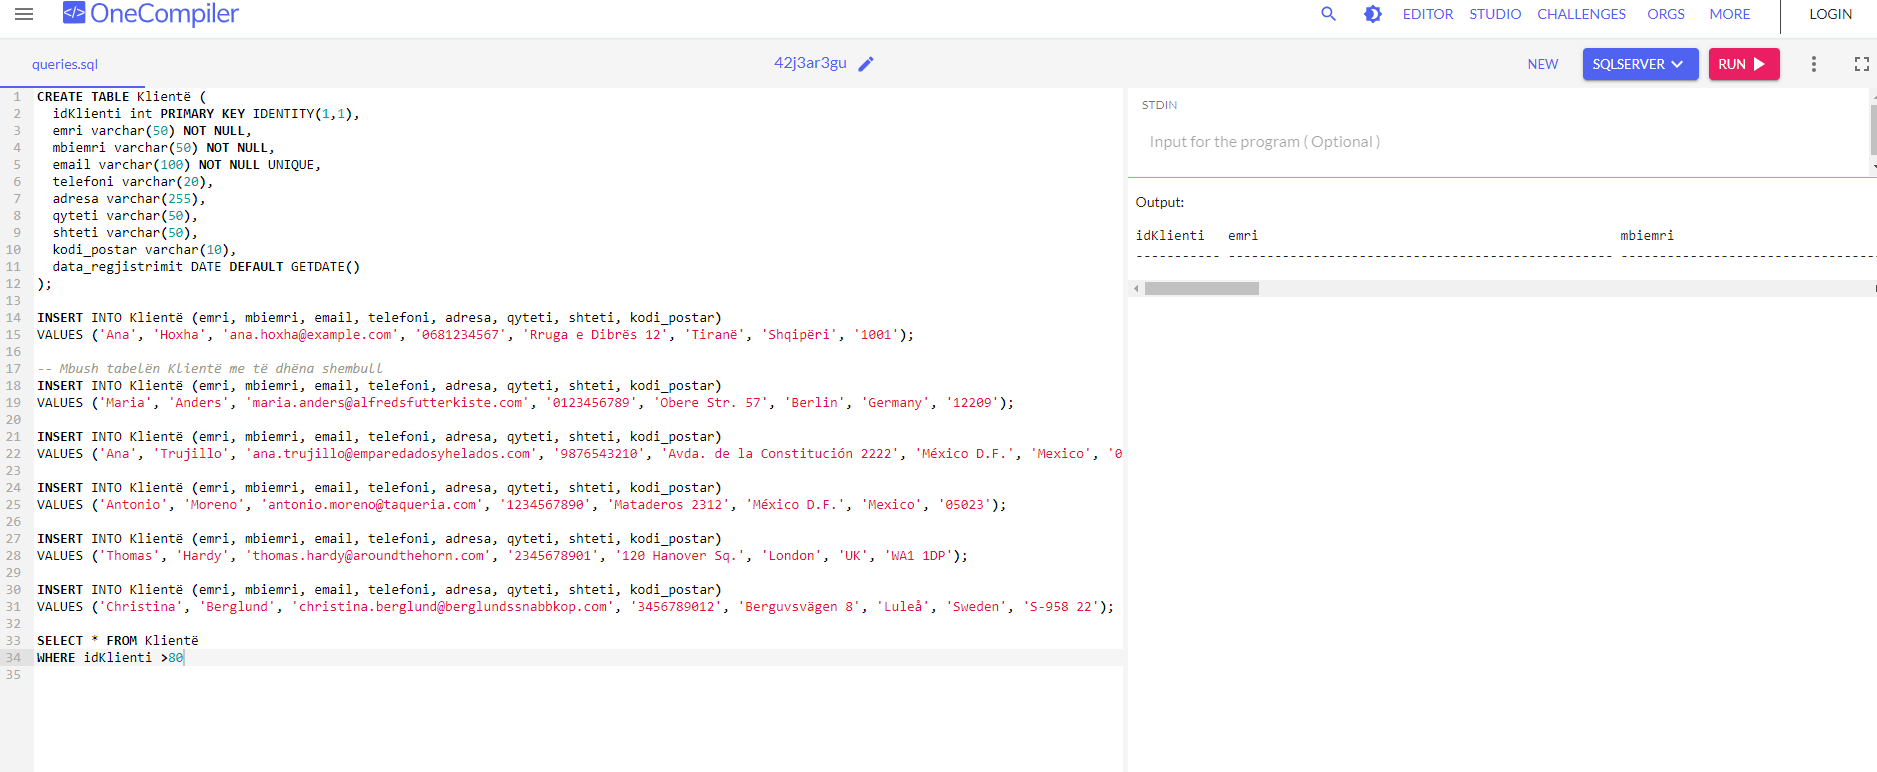
\includegraphics{./Figs/query8.png}
\end{frame}

\begin{frame}{Fjala kyç ORDER BY}
\phantomsection\label{fjala-kyuxe7-order-by}
Fjala kyç ORDER BY përdoret për të renditur grupin e rezultateve në rend
rritës ose zbritës.
\end{frame}

\begin{frame}[fragile]{Fillojmë me një tabelë}
\phantomsection\label{fillojmuxeb-me-njuxeb-tabeluxeb-2}
\AddToHookNext{env/Highlighting/begin}{\tiny}

\begin{Shaded}
\begin{Highlighting}[]
\CommentTok{{-}{-} Krijo tabelën Produkte}
\KeywordTok{CREATE} \KeywordTok{TABLE}\NormalTok{ Produkte (}
\NormalTok{  idProdukt }\DataTypeTok{int} \KeywordTok{PRIMARY} \KeywordTok{KEY}\NormalTok{ IDENTITY(}\DecValTok{1}\NormalTok{,}\DecValTok{1}\NormalTok{),}
\NormalTok{  Emri }\DataTypeTok{varchar}\NormalTok{(}\DecValTok{50}\NormalTok{) }\KeywordTok{NOT} \KeywordTok{NULL}\NormalTok{,}
\NormalTok{  Kategoria }\DataTypeTok{varchar}\NormalTok{(}\DecValTok{50}\NormalTok{),}
\NormalTok{  Cmimi }\DataTypeTok{decimal}\NormalTok{(}\DecValTok{10}\NormalTok{, }\DecValTok{2}\NormalTok{)}
\NormalTok{);}
\end{Highlighting}
\end{Shaded}
\end{frame}

\begin{frame}[fragile]{Fillojmë me një tabelë}
\phantomsection\label{fillojmuxeb-me-njuxeb-tabeluxeb-3}
\AddToHookNext{env/Highlighting/begin}{\tiny}

\begin{Shaded}
\begin{Highlighting}[]
\CommentTok{{-}{-} Mbush tabelën Produkte me të dhëna shembull}
\KeywordTok{INSERT} \KeywordTok{INTO}\NormalTok{ Produkte (Emri, Kategoria, Cmimi)}
\KeywordTok{VALUES}\NormalTok{ (}\StringTok{\textquotesingle{}Laptop\textquotesingle{}}\NormalTok{, }\StringTok{\textquotesingle{}Elektronikë\textquotesingle{}}\NormalTok{, }\FloatTok{700.00}\NormalTok{);}

\KeywordTok{INSERT} \KeywordTok{INTO}\NormalTok{ Produkte (Emri, Kategoria, Cmimi)}
\KeywordTok{VALUES}\NormalTok{ (}\StringTok{\textquotesingle{}Telefon\textquotesingle{}}\NormalTok{, }\StringTok{\textquotesingle{}Elektronikë\textquotesingle{}}\NormalTok{, }\FloatTok{300.00}\NormalTok{);}

\KeywordTok{INSERT} \KeywordTok{INTO}\NormalTok{ Produkte (Emri, Kategoria, Cmimi)}
\KeywordTok{VALUES}\NormalTok{ (}\StringTok{\textquotesingle{}Televizor\textquotesingle{}}\NormalTok{, }\StringTok{\textquotesingle{}Elektronikë\textquotesingle{}}\NormalTok{, }\FloatTok{400.00}\NormalTok{);}

\KeywordTok{INSERT} \KeywordTok{INTO}\NormalTok{ Produkte (Emri, Kategoria, Cmimi)}
\KeywordTok{VALUES}\NormalTok{ (}\StringTok{\textquotesingle{}Frigorifer\textquotesingle{}}\NormalTok{, }\StringTok{\textquotesingle{}Elektroshtëpiake\textquotesingle{}}\NormalTok{, }\FloatTok{600.00}\NormalTok{);}

\KeywordTok{INSERT} \KeywordTok{INTO}\NormalTok{ Produkte (Emri, Kategoria, Cmimi)}
\KeywordTok{VALUES}\NormalTok{ (}\StringTok{\textquotesingle{}Fshesë me korrent\textquotesingle{}}\NormalTok{, }\StringTok{\textquotesingle{}Elektroshtëpiake\textquotesingle{}}\NormalTok{, }\FloatTok{150.00}\NormalTok{);}

\CommentTok{{-}{-} Kryej SELECT për të marrë të gjitha produktet të renditura sipas çmimit}
\KeywordTok{SELECT} \OperatorTok{*} \KeywordTok{FROM}\NormalTok{ Produkte}
\KeywordTok{ORDER} \KeywordTok{BY}\NormalTok{ Cmimi;}
\end{Highlighting}
\end{Shaded}
\end{frame}

\begin{frame}{Shembull}
\phantomsection\label{shembull-8}
Renditni produktet sipas çmimit:
\end{frame}

\begin{frame}[fragile]{Shembull}
\phantomsection\label{shembull-9}
\begin{Shaded}
\begin{Highlighting}[]
\KeywordTok{SELECT} \OperatorTok{*} \KeywordTok{FROM}\NormalTok{ Produkte}
\KeywordTok{ORDER} \KeywordTok{BY}\NormalTok{ Cmimi;}
\end{Highlighting}
\end{Shaded}
\end{frame}

\begin{frame}{Shembull}
\phantomsection\label{shembull-10}
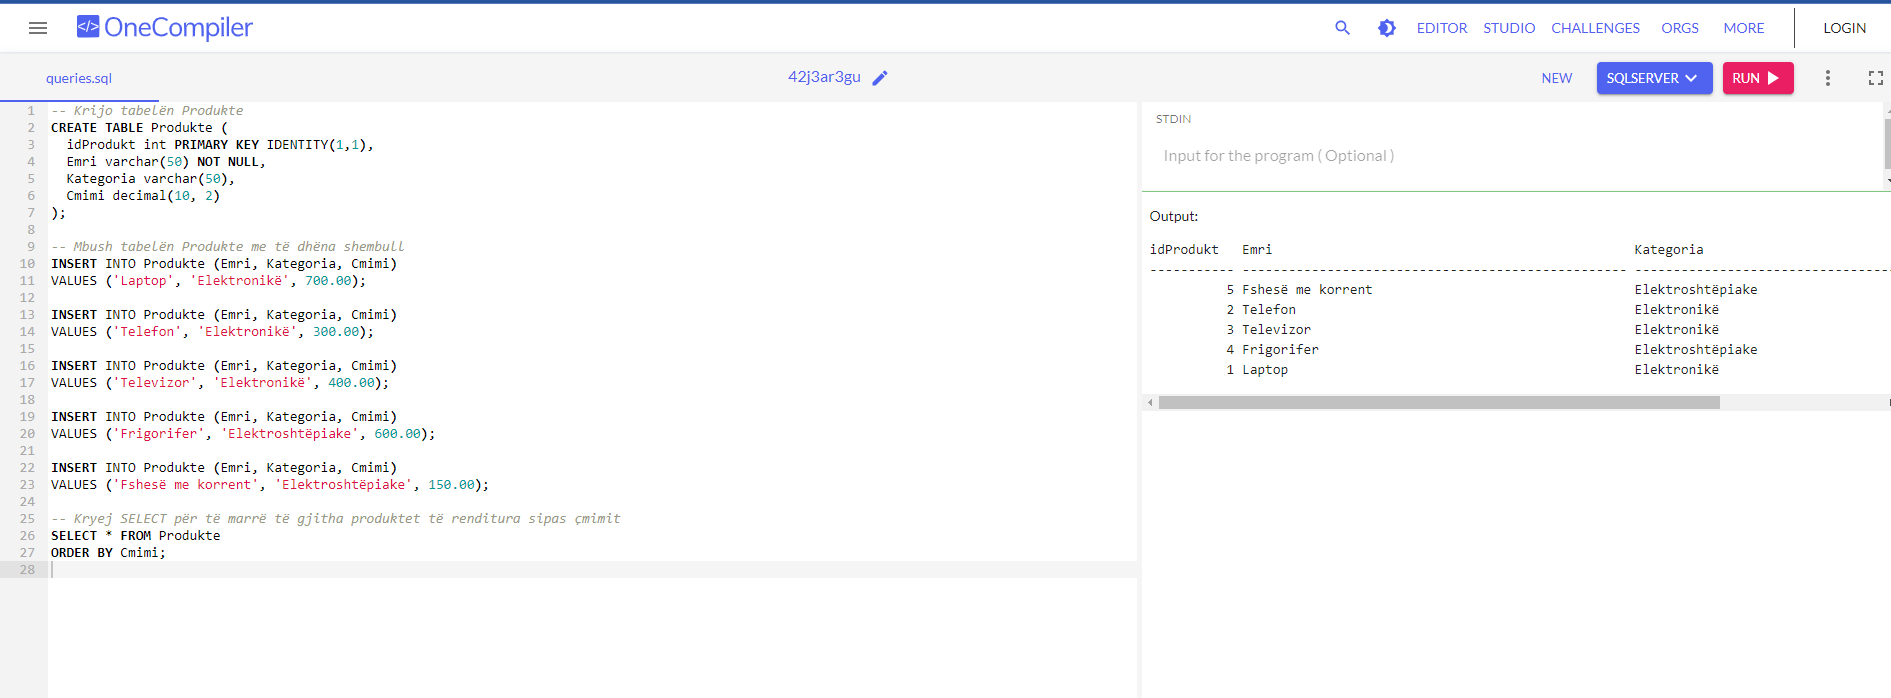
\includegraphics{./Figs/query9.png}
\end{frame}

\begin{frame}{DESC}
\phantomsection\label{desc}
\begin{itemize}
\item
  Fjala kyçe ORDER BY i rendit të dhënat në rend rritës si parazgjedhje.
\item
  Për të renditur të dhënat në rend zbritës, përdorni fjalën kyçe DESC.
\end{itemize}
\end{frame}

\begin{frame}{Shembull}
\phantomsection\label{shembull-11}
Renditni produktet nga çmimi më i lartë tek ai më i ulët:
\end{frame}

\begin{frame}[fragile]{Shembull}
\phantomsection\label{shembull-12}
\begin{Shaded}
\begin{Highlighting}[]
\KeywordTok{SELECT} \OperatorTok{*} \KeywordTok{FROM}\NormalTok{ Produkte}
\KeywordTok{ORDER} \KeywordTok{BY}\NormalTok{ Cmimi }\KeywordTok{DESC}\NormalTok{;}
\end{Highlighting}
\end{Shaded}
\end{frame}

\begin{frame}{Shembull}
\phantomsection\label{shembull-13}
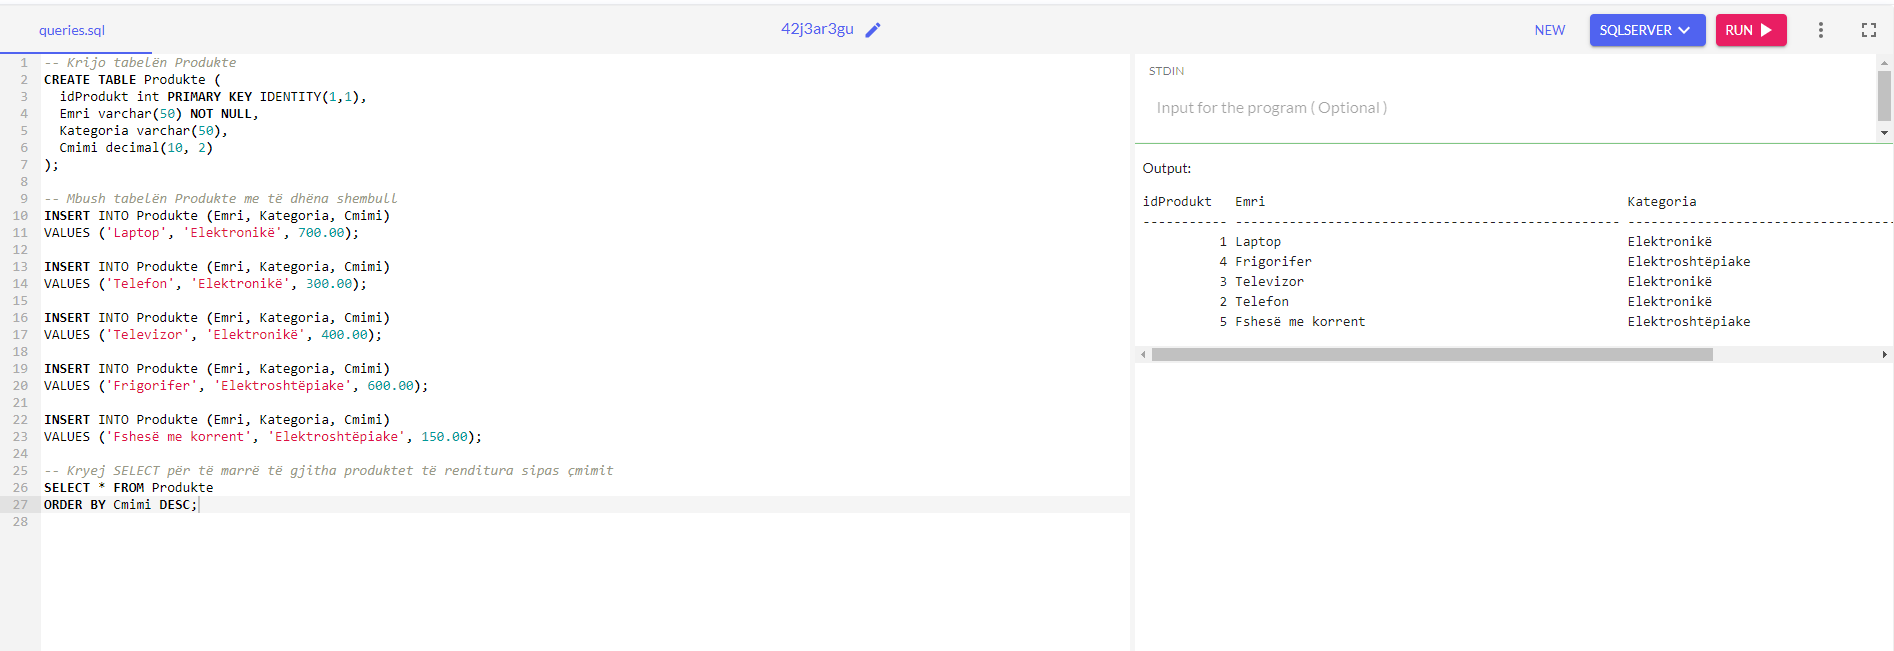
\includegraphics{./Figs/query10.png}
\end{frame}

\begin{frame}{Alfabetikisht DESC}
\phantomsection\label{alfabetikisht-desc}
\begin{itemize}
\tightlist
\item
  Për të renditur tabelën në mënyrë alfabetike nga e kundërta, përdorni
  fjalën kyçe DESC:
\end{itemize}
\end{frame}

\begin{frame}{Shembull}
\phantomsection\label{shembull-14}
\begin{itemize}
\tightlist
\item
  Renditni produktet sipas emrit të produktit në rend të kundërt:
\end{itemize}
\end{frame}

\begin{frame}[fragile]{Shembull}
\phantomsection\label{shembull-15}
\begin{Shaded}
\begin{Highlighting}[]
\KeywordTok{SELECT} \OperatorTok{*} \KeywordTok{FROM}\NormalTok{ Produkte}
\KeywordTok{ORDER} \KeywordTok{BY}\NormalTok{ Emri }\KeywordTok{DESC}\NormalTok{;}
\end{Highlighting}
\end{Shaded}
\end{frame}

\begin{frame}{Shembull}
\phantomsection\label{shembull-16}
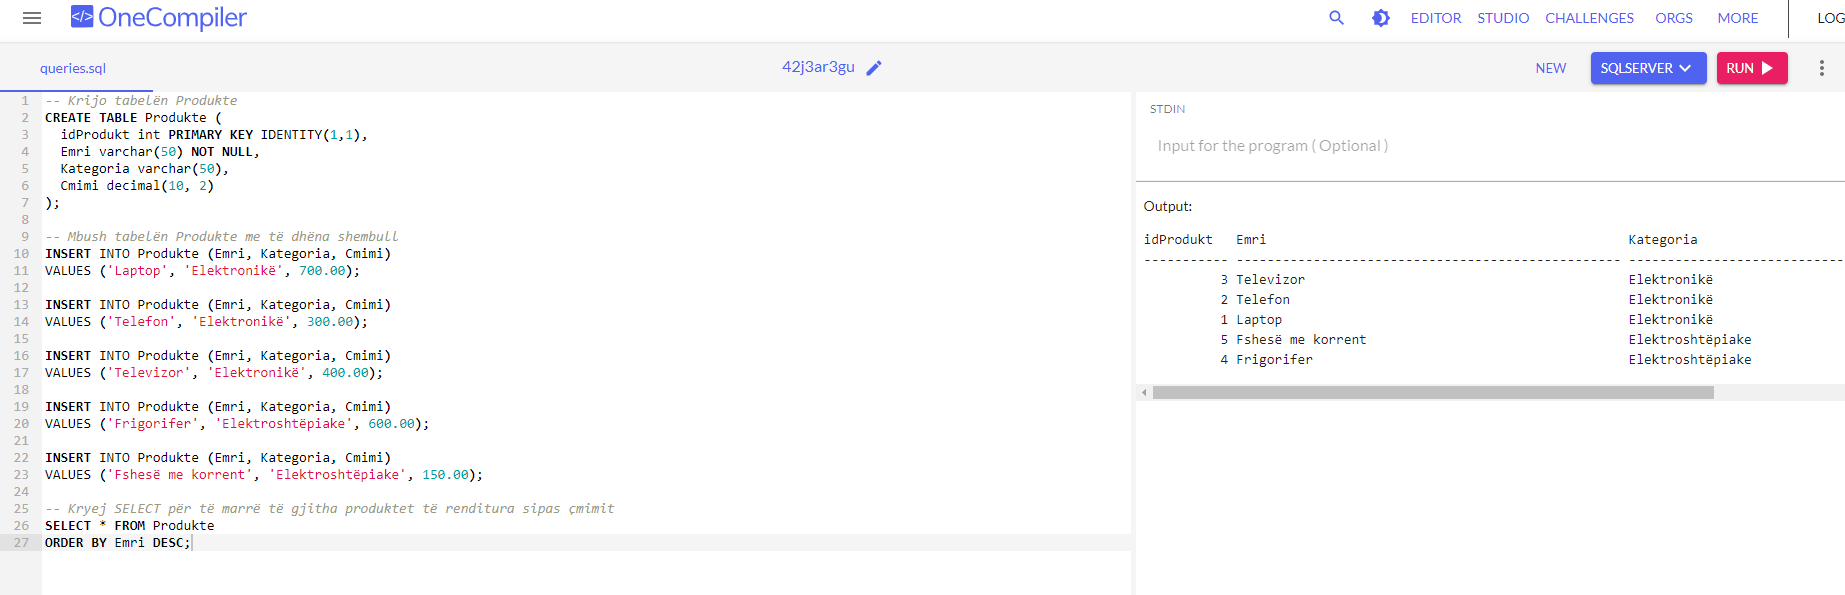
\includegraphics{./Figs/query11.png}
\end{frame}

\begin{frame}{RENDIT ME disa kolona}
\phantomsection\label{rendit-me-disa-kolona}
\begin{itemize}
\item
  Deklarata e mëposhtme SQL zgjedh të gjithë klientët nga tabela
  ``Klientë'', të renditur sipas kolonës ``Shteti'' dhe ``Emri i
  klientit''.
\item
  Kjo do të thotë se renditet sipas vendit, por nëse disa rreshta kanë
  të njëjtin shtet, ai i rendit sipas Emrit të Klientit:
\end{itemize}
\end{frame}

\begin{frame}[fragile]{Shembull}
\phantomsection\label{shembull-17}
\begin{Shaded}
\begin{Highlighting}[]
\KeywordTok{SELECT} \OperatorTok{*} \KeywordTok{FROM}\NormalTok{ Klientë}
\KeywordTok{ORDER} \KeywordTok{BY}\NormalTok{ shteti, emri;}
\end{Highlighting}
\end{Shaded}
\end{frame}

\begin{frame}{Shembull}
\phantomsection\label{shembull-18}
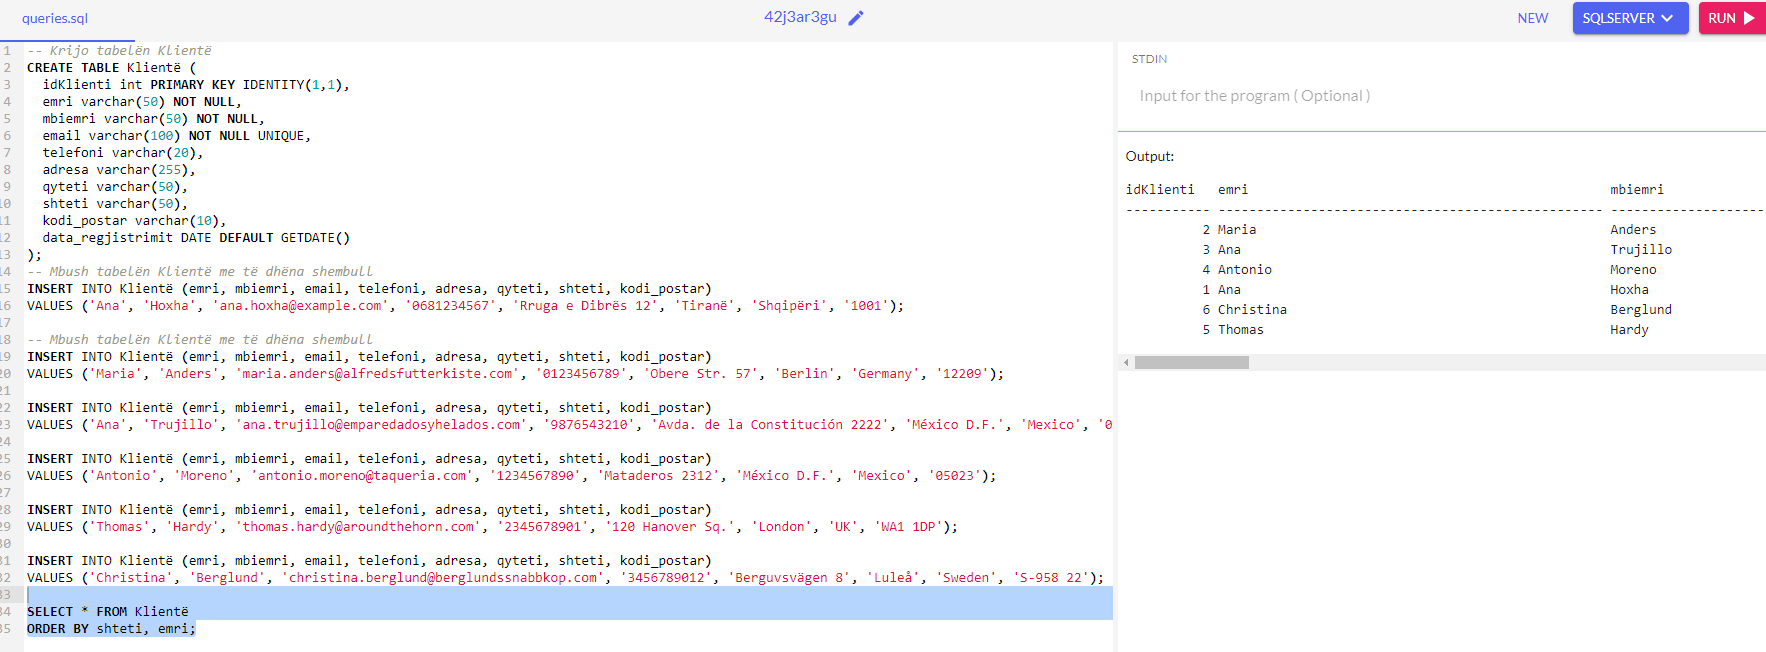
\includegraphics{./Figs/query12.png}
\end{frame}

\begin{frame}{Përdorimi bashkë i ASC dhe DESC}
\phantomsection\label{puxebrdorimi-bashkuxeb-i-asc-dhe-desc}
Deklarata e mëposhtme SQL zgjedh të gjithë klientët nga tabela
``Klientë'', të renditur në rritje sipas ``shteti'' dhe duke zbritur
sipas kolonës ``Emri i klientit'':
\end{frame}

\begin{frame}[fragile]{Shembull}
\phantomsection\label{shembull-19}
\begin{Shaded}
\begin{Highlighting}[]
\KeywordTok{SELECT} \OperatorTok{*} \KeywordTok{FROM}\NormalTok{ Klientë}
\KeywordTok{ORDER} \KeywordTok{BY}\NormalTok{ shteti, emri;}
\end{Highlighting}
\end{Shaded}
\end{frame}

\begin{frame}{Shembull}
\phantomsection\label{shembull-20}
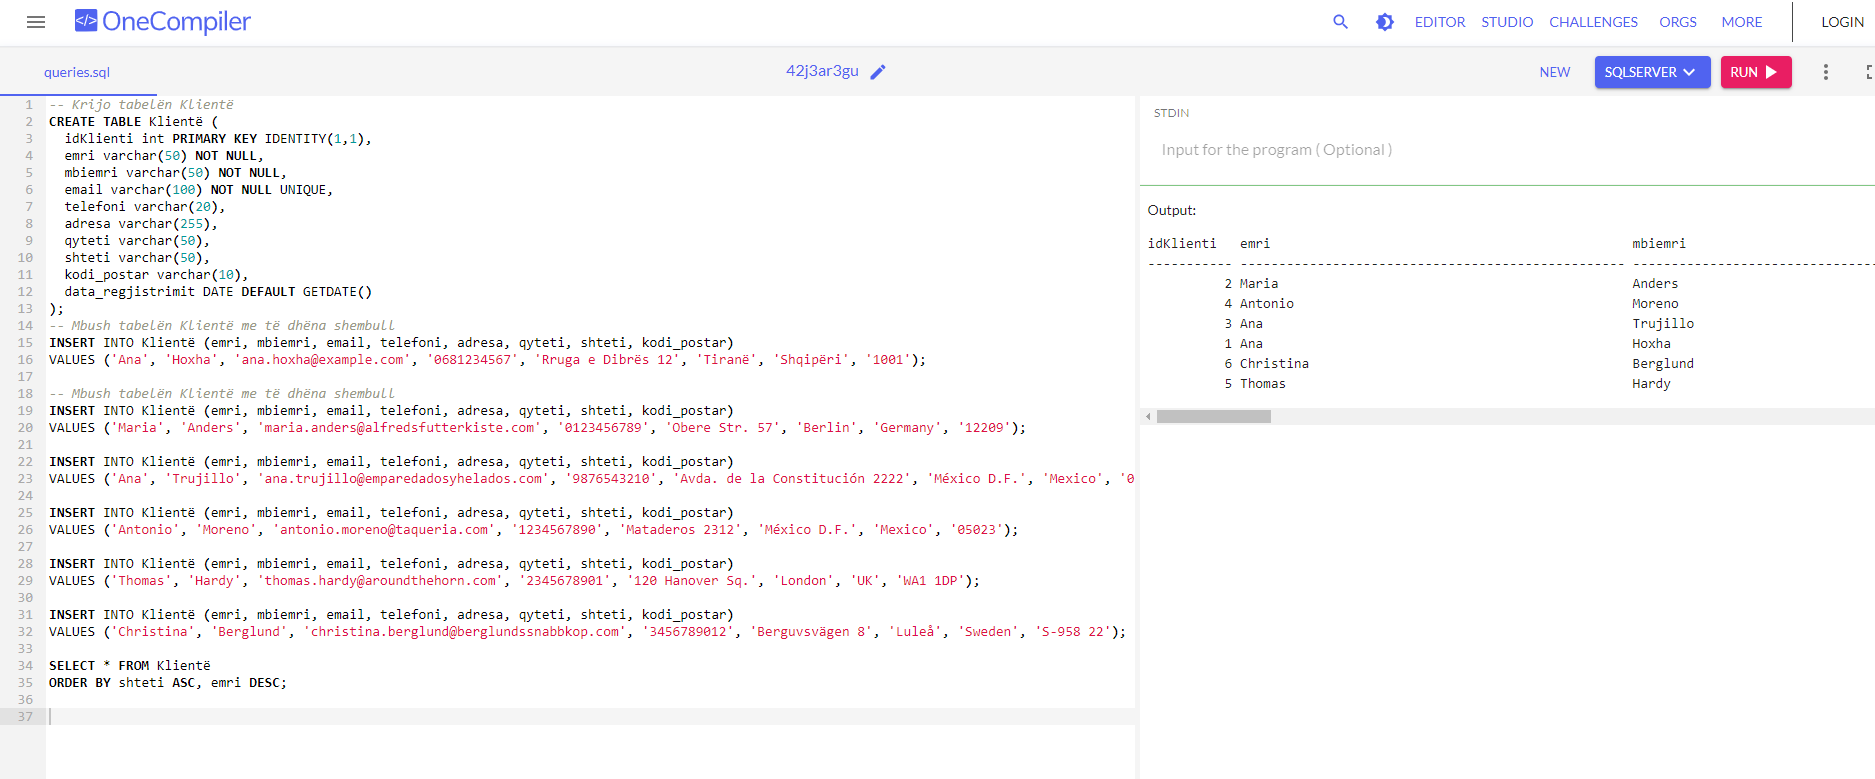
\includegraphics{./Figs/query13.png}
\end{frame}

\begin{frame}{Operatori AND}
\phantomsection\label{operatori-and}
\begin{itemize}
\item
  Klauzola WHERE mund të përmbajë një ose shumë operatorë AND.
\item
  Operatori AND përdoret për të filtruar të dhënat bazuar në më shumë se
  një kusht, si p.sh. nëse doni të ktheni të gjithë klientët nga Spanja
  që fillon me shkronjën ``G''
\end{itemize}
\end{frame}

\begin{frame}[fragile]{Fillojmë me një tabelë}
\phantomsection\label{fillojmuxeb-me-njuxeb-tabeluxeb-4}
\AddToHookNext{env/Highlighting/begin}{\tiny}

\begin{Shaded}
\begin{Highlighting}[]
\CommentTok{{-}{-} Krijo tabelën Klientë}
\KeywordTok{CREATE} \KeywordTok{TABLE}\NormalTok{ Klientë (}
\NormalTok{  idKlienti }\DataTypeTok{int} \KeywordTok{PRIMARY} \KeywordTok{KEY}\NormalTok{ IDENTITY(}\DecValTok{1}\NormalTok{,}\DecValTok{1}\NormalTok{),}
\NormalTok{  emri }\DataTypeTok{varchar}\NormalTok{(}\DecValTok{50}\NormalTok{) }\KeywordTok{NOT} \KeywordTok{NULL}\NormalTok{,}
\NormalTok{  mbiemri }\DataTypeTok{varchar}\NormalTok{(}\DecValTok{50}\NormalTok{) }\KeywordTok{NOT} \KeywordTok{NULL}\NormalTok{,}
\NormalTok{  email }\DataTypeTok{varchar}\NormalTok{(}\DecValTok{100}\NormalTok{) }\KeywordTok{NOT} \KeywordTok{NULL} \KeywordTok{UNIQUE}\NormalTok{,}
\NormalTok{  telefoni }\DataTypeTok{varchar}\NormalTok{(}\DecValTok{20}\NormalTok{),}
\NormalTok{  adresa }\DataTypeTok{varchar}\NormalTok{(}\DecValTok{255}\NormalTok{),}
\NormalTok{  qyteti }\DataTypeTok{varchar}\NormalTok{(}\DecValTok{50}\NormalTok{),}
\NormalTok{  shteti }\DataTypeTok{varchar}\NormalTok{(}\DecValTok{50}\NormalTok{),}
\NormalTok{  kodi\_postar }\DataTypeTok{varchar}\NormalTok{(}\DecValTok{10}\NormalTok{),}
\NormalTok{  data\_regjistrimit }\DataTypeTok{DATE} \KeywordTok{DEFAULT}\NormalTok{ GETDATE()}
\NormalTok{);}
\end{Highlighting}
\end{Shaded}
\end{frame}

\begin{frame}[fragile]{Fillojmë me një tabelë}
\phantomsection\label{fillojmuxeb-me-njuxeb-tabeluxeb-5}
\AddToHookNext{env/Highlighting/begin}{\tiny}

\begin{Shaded}
\begin{Highlighting}[]
\CommentTok{{-}{-} Mbush tabelën Klientë me të dhëna shembull}
\KeywordTok{INSERT} \KeywordTok{INTO}\NormalTok{ Klientë (emri, mbiemri, email, telefoni, adresa, qyteti, shteti, kodi\_postar)}
\KeywordTok{VALUES}\NormalTok{ (}\StringTok{\textquotesingle{}Ana\textquotesingle{}}\NormalTok{, }\StringTok{\textquotesingle{}Hoxha\textquotesingle{}}\NormalTok{, }\StringTok{\textquotesingle{}ana.hoxha@example.com\textquotesingle{}}\NormalTok{, }\StringTok{\textquotesingle{}0681234567\textquotesingle{}}\NormalTok{, }\StringTok{\textquotesingle{}Rruga e Dibrës 12\textquotesingle{}}\NormalTok{, }\StringTok{\textquotesingle{}Tiranë\textquotesingle{}}\NormalTok{, }\StringTok{\textquotesingle{}Shqipëri\textquotesingle{}}\NormalTok{, }\StringTok{\textquotesingle{}1001\textquotesingle{}}\NormalTok{);}

\KeywordTok{INSERT} \KeywordTok{INTO}\NormalTok{ Klientë (emri, mbiemri, email, telefoni, adresa, qyteti, shteti, kodi\_postar)}
\KeywordTok{VALUES}\NormalTok{ (}\StringTok{\textquotesingle{}Bledi\textquotesingle{}}\NormalTok{, }\StringTok{\textquotesingle{}Kola\textquotesingle{}}\NormalTok{, }\StringTok{\textquotesingle{}bledi.kola@example.com\textquotesingle{}}\NormalTok{, }\StringTok{\textquotesingle{}0697654321\textquotesingle{}}\NormalTok{, }\StringTok{\textquotesingle{}Bulevardi Zogu I 45\textquotesingle{}}\NormalTok{, }\StringTok{\textquotesingle{}Durrës\textquotesingle{}}\NormalTok{, }\StringTok{\textquotesingle{}Shqipëri\textquotesingle{}}\NormalTok{, }\StringTok{\textquotesingle{}2002\textquotesingle{}}\NormalTok{);}

\KeywordTok{INSERT} \KeywordTok{INTO}\NormalTok{ Klientë (emri, mbiemri, email, telefoni, adresa, qyteti, shteti, kodi\_postar)}
\KeywordTok{VALUES}\NormalTok{ (}\StringTok{\textquotesingle{}Elira\textquotesingle{}}\NormalTok{, }\StringTok{\textquotesingle{}Dervishi\textquotesingle{}}\NormalTok{, }\StringTok{\textquotesingle{}elira.dervishi@example.com\textquotesingle{}}\NormalTok{, }\StringTok{\textquotesingle{}0687654321\textquotesingle{}}\NormalTok{, }\StringTok{\textquotesingle{}Rruga Myslym Shyri 88\textquotesingle{}}\NormalTok{, }\StringTok{\textquotesingle{}Tiranë\textquotesingle{}}\NormalTok{, }\StringTok{\textquotesingle{}Shqipëri\textquotesingle{}}\NormalTok{, }\StringTok{\textquotesingle{}1001\textquotesingle{}}\NormalTok{);}

\KeywordTok{INSERT} \KeywordTok{INTO}\NormalTok{ Klientë (emri, mbiemri, email, telefoni, adresa, qyteti, shteti, kodi\_postar)}
\KeywordTok{VALUES}\NormalTok{ (}\StringTok{\textquotesingle{}Arjan\textquotesingle{}}\NormalTok{, }\StringTok{\textquotesingle{}Lika\textquotesingle{}}\NormalTok{, }\StringTok{\textquotesingle{}arjan.lika@example.com\textquotesingle{}}\NormalTok{, }\StringTok{\textquotesingle{}0671234567\textquotesingle{}}\NormalTok{, }\StringTok{\textquotesingle{}Rruga e Kavajës 23\textquotesingle{}}\NormalTok{, }\StringTok{\textquotesingle{}Vlorë\textquotesingle{}}\NormalTok{, }\StringTok{\textquotesingle{}Shqipëri\textquotesingle{}}\NormalTok{, }\StringTok{\textquotesingle{}3003\textquotesingle{}}\NormalTok{);}

\KeywordTok{INSERT} \KeywordTok{INTO}\NormalTok{ Klientë (emri, mbiemri, email, telefoni, adresa, qyteti, shteti, kodi\_postar)}
\KeywordTok{VALUES}\NormalTok{ (}\StringTok{\textquotesingle{}Diana\textquotesingle{}}\NormalTok{, }\StringTok{\textquotesingle{}Mema\textquotesingle{}}\NormalTok{, }\StringTok{\textquotesingle{}diana.mema@example.com\textquotesingle{}}\NormalTok{, }\StringTok{\textquotesingle{}0691234567\textquotesingle{}}\NormalTok{, }\StringTok{\textquotesingle{}Bulevardi Dëshmorët e Kombit 7\textquotesingle{}}\NormalTok{, }\StringTok{\textquotesingle{}Shkodër\textquotesingle{}}\NormalTok{, }\StringTok{\textquotesingle{}Shqipëri\textquotesingle{}}\NormalTok{, }\StringTok{\textquotesingle{}4004\textquotesingle{}}\NormalTok{);}

\KeywordTok{INSERT} \KeywordTok{INTO}\NormalTok{ Klientë (emri, mbiemri, email, telefoni, adresa, qyteti, shteti, kodi\_postar)}
\KeywordTok{VALUES}\NormalTok{ (}\StringTok{\textquotesingle{}Gabriel\textquotesingle{}}\NormalTok{, }\StringTok{\textquotesingle{}Garcia\textquotesingle{}}\NormalTok{, }\StringTok{\textquotesingle{}gabriel.garcia@example.com\textquotesingle{}}\NormalTok{, }\StringTok{\textquotesingle{}0698765432\textquotesingle{}}\NormalTok{, }\StringTok{\textquotesingle{}Calle Mayor 5\textquotesingle{}}\NormalTok{, }\StringTok{\textquotesingle{}Madrid\textquotesingle{}}\NormalTok{, }\StringTok{\textquotesingle{}Spain\textquotesingle{}}\NormalTok{, }\StringTok{\textquotesingle{}28013\textquotesingle{}}\NormalTok{);}

\KeywordTok{INSERT} \KeywordTok{INTO}\NormalTok{ Klientë (emri, mbiemri, email, telefoni, adresa, qyteti, shteti, kodi\_postar)}
\KeywordTok{VALUES}\NormalTok{ (}\StringTok{\textquotesingle{}Gonzalo\textquotesingle{}}\NormalTok{, }\StringTok{\textquotesingle{}Perez\textquotesingle{}}\NormalTok{, }\StringTok{\textquotesingle{}gonzalo.perez@example.com\textquotesingle{}}\NormalTok{, }\StringTok{\textquotesingle{}0687654321\textquotesingle{}}\NormalTok{, }\StringTok{\textquotesingle{}Gran Via 12\textquotesingle{}}\NormalTok{, }\StringTok{\textquotesingle{}Barcelona\textquotesingle{}}\NormalTok{, }\StringTok{\textquotesingle{}Spain\textquotesingle{}}\NormalTok{, }\StringTok{\textquotesingle{}08010\textquotesingle{}}\NormalTok{);}

\KeywordTok{INSERT} \KeywordTok{INTO}\NormalTok{ Klientë (emri, mbiemri, email, telefoni, adresa, qyteti, shteti, kodi\_postar)}
\KeywordTok{VALUES}\NormalTok{ (}\StringTok{\textquotesingle{}Maria\textquotesingle{}}\NormalTok{, }\StringTok{\textquotesingle{}Anders\textquotesingle{}}\NormalTok{, }\StringTok{\textquotesingle{}maria.anders@example.com\textquotesingle{}}\NormalTok{, }\StringTok{\textquotesingle{}0123456789\textquotesingle{}}\NormalTok{, }\StringTok{\textquotesingle{}Obere Str. 57\textquotesingle{}}\NormalTok{, }\StringTok{\textquotesingle{}Berlin\textquotesingle{}}\NormalTok{, }\StringTok{\textquotesingle{}Germany\textquotesingle{}}\NormalTok{, }\StringTok{\textquotesingle{}12209\textquotesingle{}}\NormalTok{);}

\KeywordTok{INSERT} \KeywordTok{INTO}\NormalTok{ Klientë (emri, mbiemri, email, telefoni, adresa, qyteti, shteti, kodi\_postar)}
\KeywordTok{VALUES}\NormalTok{ (}\StringTok{\textquotesingle{}Thomas\textquotesingle{}}\NormalTok{, }\StringTok{\textquotesingle{}Hardy\textquotesingle{}}\NormalTok{, }\StringTok{\textquotesingle{}thomas.hardy@example.com\textquotesingle{}}\NormalTok{, }\StringTok{\textquotesingle{}2345678901\textquotesingle{}}\NormalTok{, }\StringTok{\textquotesingle{}120 Hanover Sq.\textquotesingle{}}\NormalTok{, }\StringTok{\textquotesingle{}London\textquotesingle{}}\NormalTok{, }\StringTok{\textquotesingle{}UK\textquotesingle{}}\NormalTok{, }\StringTok{\textquotesingle{}WA1 1DP\textquotesingle{}}\NormalTok{);}
\end{Highlighting}
\end{Shaded}
\end{frame}

\begin{frame}{Shembull}
\phantomsection\label{shembull-21}
Zgjidhni të gjithë klientët nga Spanja që fillojnë me shkronjën ``G'':
\end{frame}

\begin{frame}[fragile]{Shembull}
\phantomsection\label{shembull-22}
\AddToHookNext{env/Highlighting/begin}{\tiny}

\begin{Shaded}
\begin{Highlighting}[]
\CommentTok{{-}{-} Kryej SELECT për të marrë të gjitha rreshtat e klientëve të renditur sipas kritereve të specifikuara}
\KeywordTok{SELECT} \OperatorTok{*} 
\KeywordTok{FROM}\NormalTok{ Klientë}
\KeywordTok{WHERE}\NormalTok{ shteti }\OperatorTok{=} \StringTok{\textquotesingle{}Spain\textquotesingle{}} \KeywordTok{AND}\NormalTok{ emri }\KeywordTok{LIKE} \StringTok{\textquotesingle{}G\%\textquotesingle{}}\NormalTok{;}
\end{Highlighting}
\end{Shaded}
\end{frame}

\begin{frame}{Shembull}
\phantomsection\label{shembull-23}
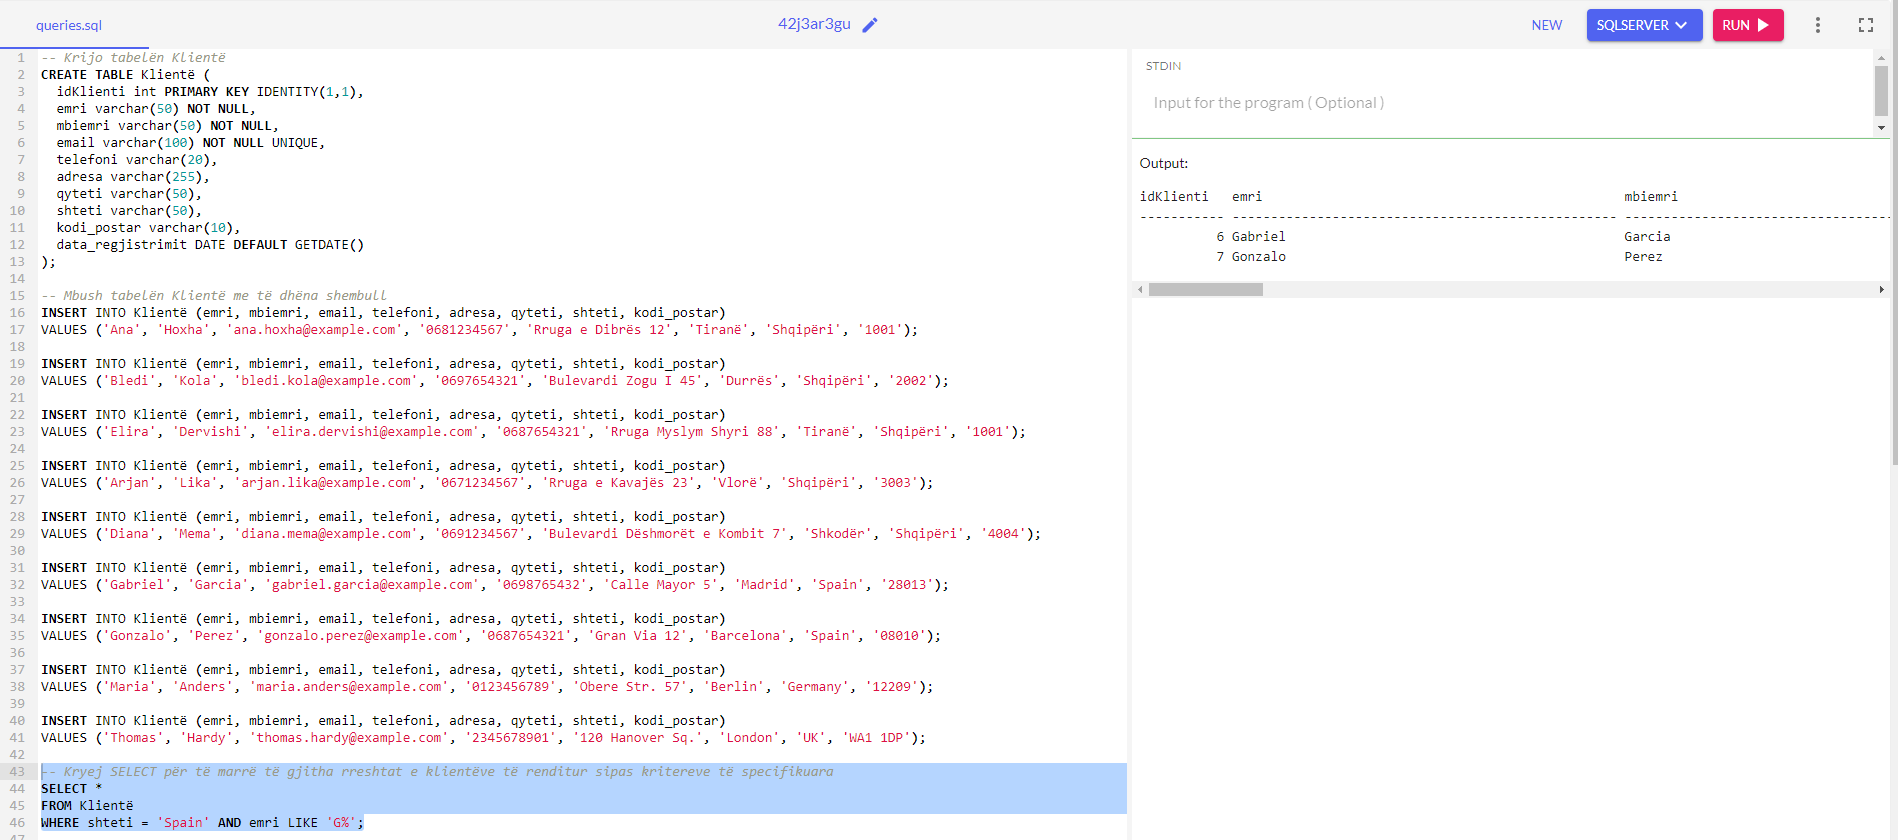
\includegraphics{./Figs/query14.png}
\end{frame}

\begin{frame}{AND vs OR}
\phantomsection\label{and-vs-or}
\begin{itemize}
\item
  Operatori AND shfaq një rekord nëse të gjitha kushtet janë të vërteta.
\item
  Operatori OR shfaq një rekord nëse ndonjë nga kushtet është e VËRTETË.
\end{itemize}
\end{frame}

\begin{frame}{Të gjitha kushtet duhet të jenë të vërteta}
\phantomsection\label{tuxeb-gjitha-kushtet-duhet-tuxeb-jenuxeb-tuxeb-vuxebrteta}
\begin{itemize}
\tightlist
\item
  Deklarata e mëposhtme SQL zgjedh të gjitha fushat nga klientët ku
  vendi është ``Gjermania'' DHE qyteti është ``Berlin'' DHE Kodi Postar
  është më i lartë se 12000:
\end{itemize}
\end{frame}

\begin{frame}[fragile]{Fillojmë me një tabelë}
\phantomsection\label{fillojmuxeb-me-njuxeb-tabeluxeb-6}
\AddToHookNext{env/Highlighting/begin}{\tiny}

\begin{Shaded}
\begin{Highlighting}[]
\CommentTok{{-}{-} Krijo tabelën Klientë}
\KeywordTok{CREATE} \KeywordTok{TABLE}\NormalTok{ Klientë (}
\NormalTok{  idKlienti }\DataTypeTok{int} \KeywordTok{PRIMARY} \KeywordTok{KEY}\NormalTok{ IDENTITY(}\DecValTok{1}\NormalTok{,}\DecValTok{1}\NormalTok{),}
\NormalTok{  emri }\DataTypeTok{varchar}\NormalTok{(}\DecValTok{50}\NormalTok{) }\KeywordTok{NOT} \KeywordTok{NULL}\NormalTok{,}
\NormalTok{  mbiemri }\DataTypeTok{varchar}\NormalTok{(}\DecValTok{50}\NormalTok{) }\KeywordTok{NOT} \KeywordTok{NULL}\NormalTok{,}
\NormalTok{  email }\DataTypeTok{varchar}\NormalTok{(}\DecValTok{100}\NormalTok{) }\KeywordTok{NOT} \KeywordTok{NULL} \KeywordTok{UNIQUE}\NormalTok{,}
\NormalTok{  telefoni }\DataTypeTok{varchar}\NormalTok{(}\DecValTok{20}\NormalTok{),}
\NormalTok{  adresa }\DataTypeTok{varchar}\NormalTok{(}\DecValTok{255}\NormalTok{),}
\NormalTok{  qyteti }\DataTypeTok{varchar}\NormalTok{(}\DecValTok{50}\NormalTok{),}
\NormalTok{  shteti }\DataTypeTok{varchar}\NormalTok{(}\DecValTok{50}\NormalTok{),}
\NormalTok{  kodi\_postar }\DataTypeTok{varchar}\NormalTok{(}\DecValTok{10}\NormalTok{),}
\NormalTok{  data\_regjistrimit }\DataTypeTok{DATE} \KeywordTok{DEFAULT}\NormalTok{ GETDATE()}
\NormalTok{);}
\end{Highlighting}
\end{Shaded}
\end{frame}

\begin{frame}[fragile]{Fillojmë me një tabelë}
\phantomsection\label{fillojmuxeb-me-njuxeb-tabeluxeb-7}
\AddToHookNext{env/Highlighting/begin}{\tiny}

\begin{Shaded}
\begin{Highlighting}[]
\CommentTok{{-}{-} Mbush tabelën Klientë me të dhëna shembull}
\KeywordTok{INSERT} \KeywordTok{INTO}\NormalTok{ Klientë (emri, mbiemri, email, telefoni, adresa, qyteti, shteti, kodi\_postar)}
\KeywordTok{VALUES}\NormalTok{ (}\StringTok{\textquotesingle{}Maria\textquotesingle{}}\NormalTok{, }\StringTok{\textquotesingle{}Anders\textquotesingle{}}\NormalTok{, }\StringTok{\textquotesingle{}maria.anders@example.com\textquotesingle{}}\NormalTok{, }\StringTok{\textquotesingle{}0123456789\textquotesingle{}}\NormalTok{, }\StringTok{\textquotesingle{}Obere Str. 57\textquotesingle{}}\NormalTok{, }\StringTok{\textquotesingle{}Berlin\textquotesingle{}}\NormalTok{, }\StringTok{\textquotesingle{}Gjermani\textquotesingle{}}\NormalTok{, }\StringTok{\textquotesingle{}12209\textquotesingle{}}\NormalTok{);}

\KeywordTok{INSERT} \KeywordTok{INTO}\NormalTok{ Klientë (emri, mbiemri, email, telefoni, adresa, qyteti, shteti, kodi\_postar)}
\KeywordTok{VALUES}\NormalTok{ (}\StringTok{\textquotesingle{}Ana\textquotesingle{}}\NormalTok{, }\StringTok{\textquotesingle{}Trujillo\textquotesingle{}}\NormalTok{, }\StringTok{\textquotesingle{}ana.trujillo@example.com\textquotesingle{}}\NormalTok{, }\StringTok{\textquotesingle{}9876543210\textquotesingle{}}\NormalTok{, }\StringTok{\textquotesingle{}Avda. de la Constitución 2222\textquotesingle{}}\NormalTok{, }\StringTok{\textquotesingle{}México D.F.\textquotesingle{}}\NormalTok{, }\StringTok{\textquotesingle{}Meksikë\textquotesingle{}}\NormalTok{, }\StringTok{\textquotesingle{}05021\textquotesingle{}}\NormalTok{);}

\KeywordTok{INSERT} \KeywordTok{INTO}\NormalTok{ Klientë (emri, mbiemri, email, telefoni, adresa, qyteti, shteti, kodi\_postar)}
\KeywordTok{VALUES}\NormalTok{ (}\StringTok{\textquotesingle{}Antonio\textquotesingle{}}\NormalTok{, }\StringTok{\textquotesingle{}Moreno\textquotesingle{}}\NormalTok{, }\StringTok{\textquotesingle{}antonio.moreno@example.com\textquotesingle{}}\NormalTok{, }\StringTok{\textquotesingle{}1234567890\textquotesingle{}}\NormalTok{, }\StringTok{\textquotesingle{}Mataderos 2312\textquotesingle{}}\NormalTok{, }\StringTok{\textquotesingle{}México D.F.\textquotesingle{}}\NormalTok{, }\StringTok{\textquotesingle{}Meksikë\textquotesingle{}}\NormalTok{, }\StringTok{\textquotesingle{}05023\textquotesingle{}}\NormalTok{);}

\KeywordTok{INSERT} \KeywordTok{INTO}\NormalTok{ Klientë (emri, mbiemri, email, telefoni, adresa, qyteti, shteti, kodi\_postar)}
\KeywordTok{VALUES}\NormalTok{ (}\StringTok{\textquotesingle{}Thomas\textquotesingle{}}\NormalTok{, }\StringTok{\textquotesingle{}Hardy\textquotesingle{}}\NormalTok{, }\StringTok{\textquotesingle{}thomas.hardy@example.com\textquotesingle{}}\NormalTok{, }\StringTok{\textquotesingle{}2345678901\textquotesingle{}}\NormalTok{, }\StringTok{\textquotesingle{}120 Hanover Sq.\textquotesingle{}}\NormalTok{, }\StringTok{\textquotesingle{}Londër\textquotesingle{}}\NormalTok{, }\StringTok{\textquotesingle{}MB\textquotesingle{}}\NormalTok{, }\StringTok{\textquotesingle{}WA1 1DP\textquotesingle{}}\NormalTok{);}

\KeywordTok{INSERT} \KeywordTok{INTO}\NormalTok{ Klientë (emri, mbiemri, email, telefoni, adresa, qyteti, shteti, kodi\_postar)}
\KeywordTok{VALUES}\NormalTok{ (}\StringTok{\textquotesingle{}Christina\textquotesingle{}}\NormalTok{, }\StringTok{\textquotesingle{}Berglund\textquotesingle{}}\NormalTok{, }\StringTok{\textquotesingle{}christina.berglund@example.com\textquotesingle{}}\NormalTok{, }\StringTok{\textquotesingle{}3456789012\textquotesingle{}}\NormalTok{, }\StringTok{\textquotesingle{}Berguvsvägen 8\textquotesingle{}}\NormalTok{, }\StringTok{\textquotesingle{}Luleå\textquotesingle{}}\NormalTok{, }\StringTok{\textquotesingle{}Suedi\textquotesingle{}}\NormalTok{, }\StringTok{\textquotesingle{}S{-}958 22\textquotesingle{}}\NormalTok{);}
\end{Highlighting}
\end{Shaded}
\end{frame}

\begin{frame}[fragile]{Shembull}
\phantomsection\label{shembull-24}
\AddToHookNext{env/Highlighting/begin}{\tiny}

\begin{Shaded}
\begin{Highlighting}[]
\CommentTok{{-}{-} Kryej SELECT për të marrë të gjitha rreshtat e klientëve që plotësojnë kushtet e specifikuara}
\KeywordTok{SELECT} \OperatorTok{*} 
\KeywordTok{FROM}\NormalTok{ Klientë}
\KeywordTok{WHERE}\NormalTok{ shteti }\OperatorTok{=} \StringTok{\textquotesingle{}Gjermani\textquotesingle{}}
\KeywordTok{AND}\NormalTok{ qyteti }\OperatorTok{=} \StringTok{\textquotesingle{}Berlin\textquotesingle{}}
\KeywordTok{AND}\NormalTok{ kodi\_postar }\OperatorTok{\textgreater{}} \StringTok{\textquotesingle{}12000\textquotesingle{}}\NormalTok{;}
\end{Highlighting}
\end{Shaded}
\end{frame}

\begin{frame}{Shembull}
\phantomsection\label{shembull-25}
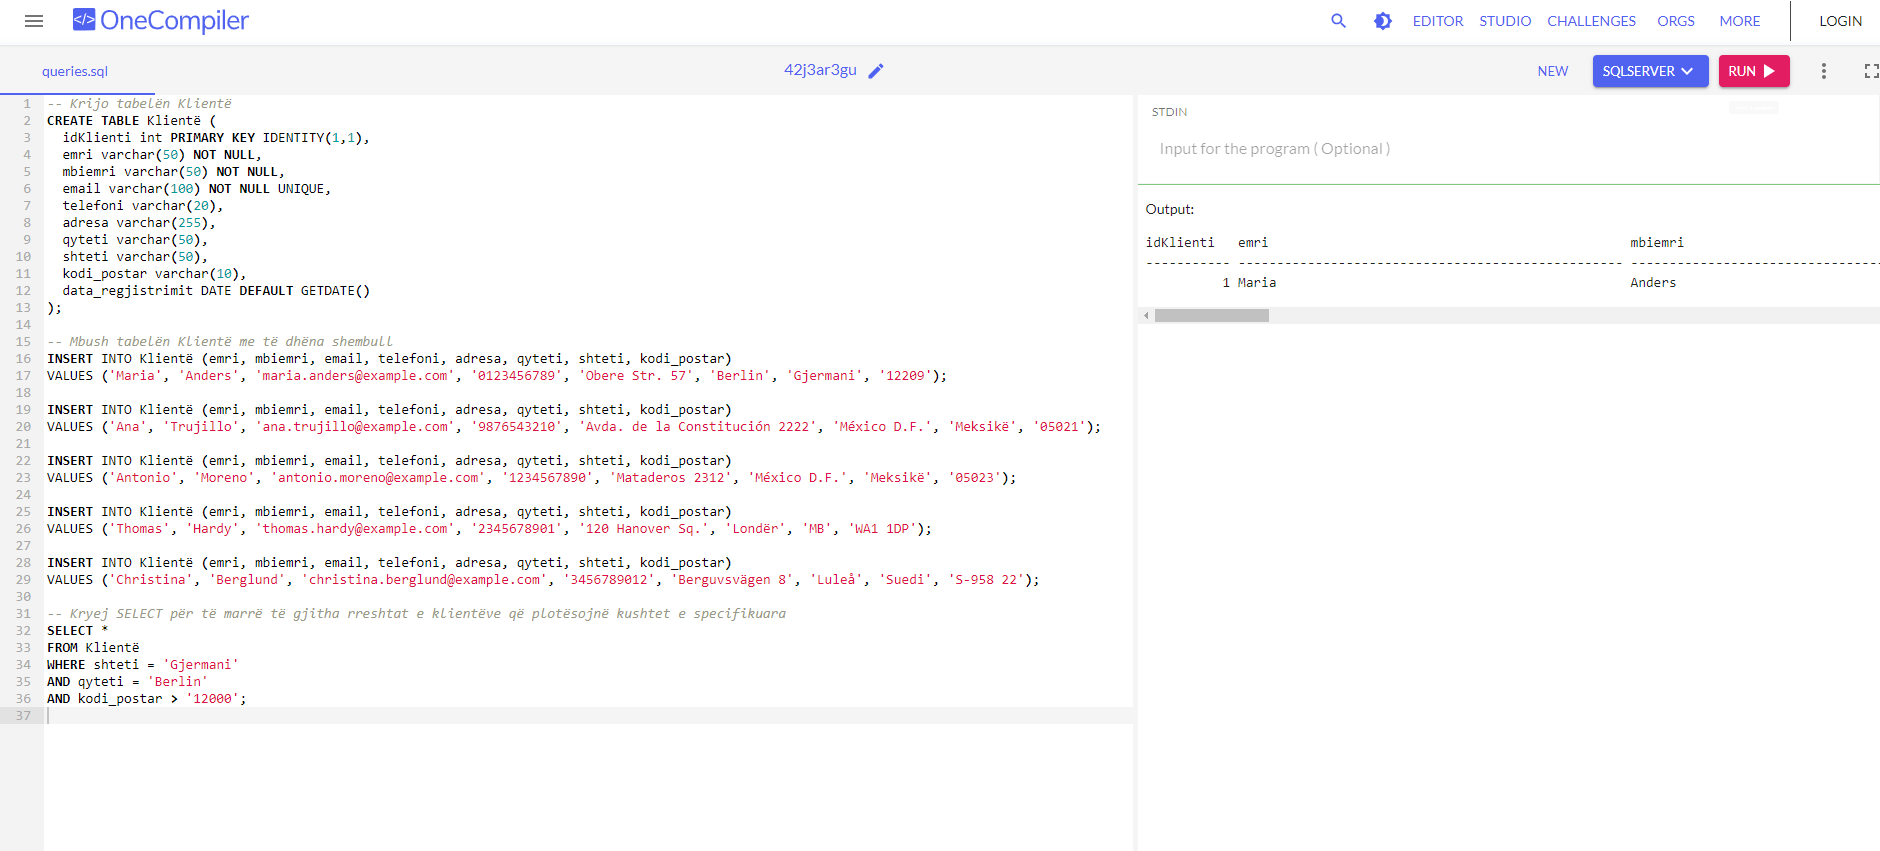
\includegraphics{./Figs/query15.png}
\end{frame}

\begin{frame}{Kombinimi AND dhe OR}
\phantomsection\label{kombinimi-and-dhe-or}
\begin{itemize}
\item
  Mund të kombinoni operatorët AND dhe OR.
\item
  Deklarata e mëposhtme SQL zgjedh të gjithë klientët nga Spanja që
  fillojnë me një ``G'' ose një ``R''.
\item
  Sigurohuni që të përdorni kllapa për të marrë rezultatin e saktë.
\end{itemize}
\end{frame}

\begin{frame}{Shembull}
\phantomsection\label{shembull-26}
Zgjidhni të gjithë klientët meksikanë që fillojnë me ``A'' ose ``M'':
\end{frame}

\begin{frame}[fragile]{Shembull}
\phantomsection\label{shembull-27}
\AddToHookNext{env/Highlighting/begin}{\tiny}

\begin{Shaded}
\begin{Highlighting}[]
\CommentTok{{-}{-} Kryej SELECT për të marrë të gjitha rreshtat e klientëve që plotësojnë kushtet e specifikuara}
\KeywordTok{SELECT} \OperatorTok{*} 
\KeywordTok{FROM}\NormalTok{ Klientë}
\KeywordTok{WHERE}\NormalTok{ shteti }\OperatorTok{=} \StringTok{\textquotesingle{}Meksikë\textquotesingle{}}
\KeywordTok{AND}\NormalTok{ (emri }\KeywordTok{LIKE} \StringTok{\textquotesingle{}A\%\textquotesingle{}} \KeywordTok{OR}\NormalTok{ emri }\KeywordTok{LIKE} \StringTok{\textquotesingle{}M\%\textquotesingle{}}\NormalTok{);}
\end{Highlighting}
\end{Shaded}
\end{frame}

\begin{frame}{Shembull}
\phantomsection\label{shembull-28}
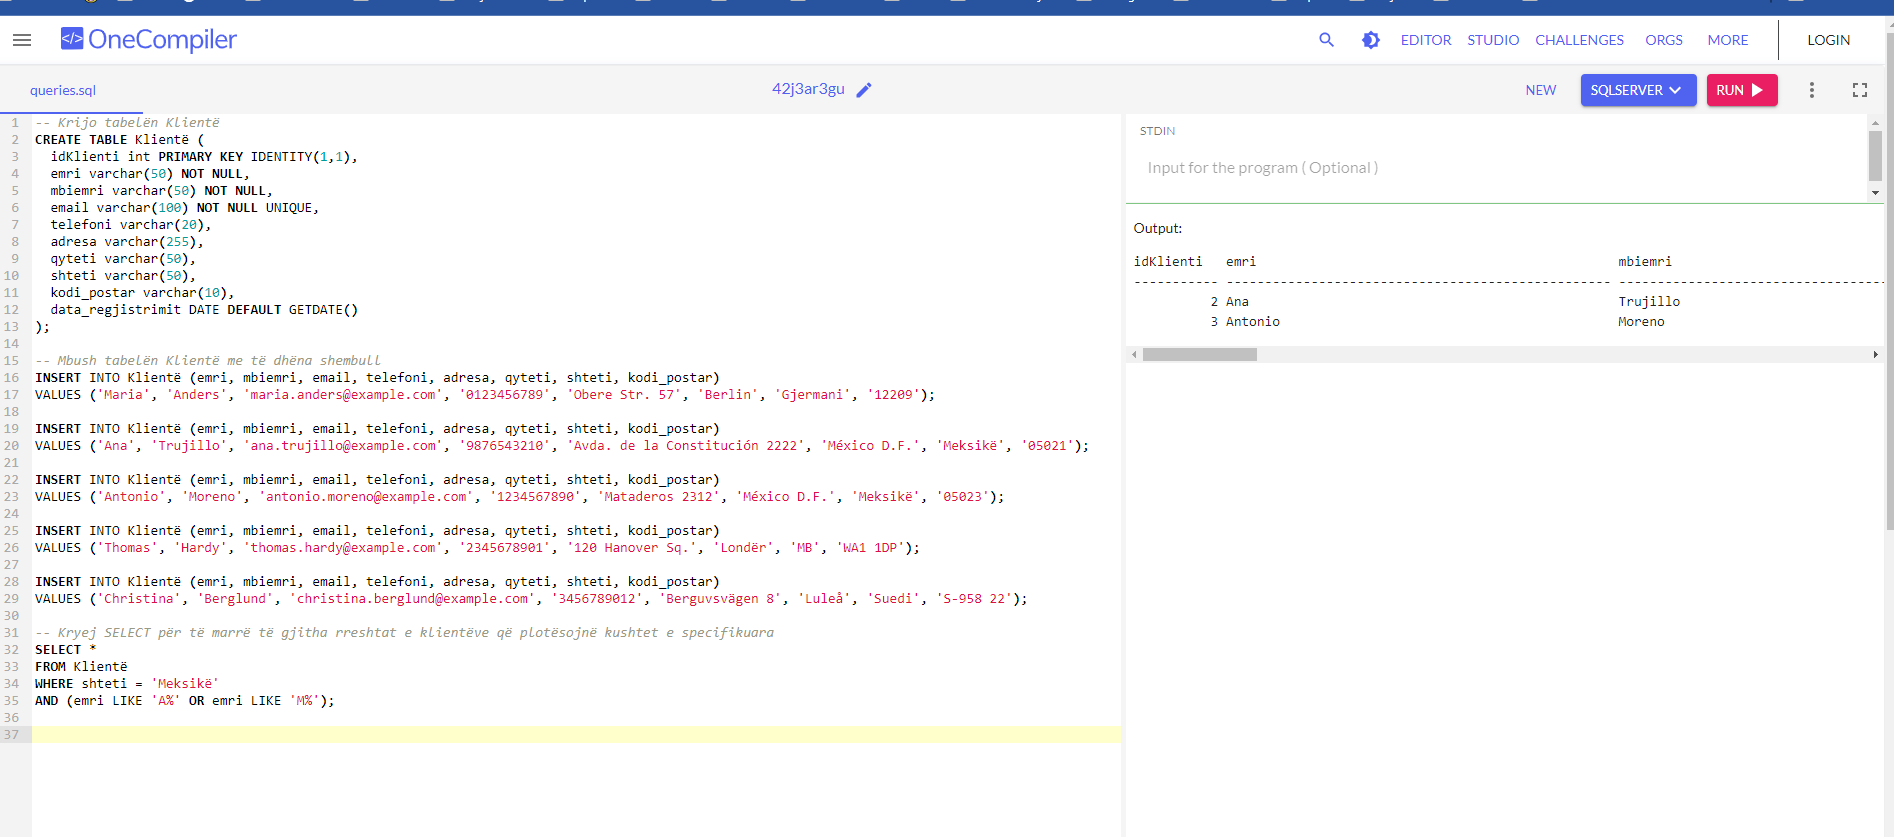
\includegraphics{./Figs/query16.png}
\end{frame}

\begin{frame}{Kombinimi AND dhe OR}
\phantomsection\label{kombinimi-and-dhe-or-1}
\begin{itemize}
\tightlist
\item
  Pa kllapa, deklarata e përzgjedhur do t'i kthejë të gjithë klientët
  nga Spanja që fillojnë me një ``A'', plus të gjithë klientët që
  fillojnë me një ``M'', pavarësisht nga vlera e vendit:
\end{itemize}
\end{frame}

\begin{frame}{Shembull}
\phantomsection\label{shembull-29}
Zgjidhni të gjithë klientët që ose:

\begin{itemize}
\tightlist
\item
  janë nga Meksika dhe fillon ose me ``A'' ose fillon me shkronjën
  ``R'':
\end{itemize}
\end{frame}

\begin{frame}[fragile]{Shembull}
\phantomsection\label{shembull-30}
\AddToHookNext{env/Highlighting/begin}{\tiny}

\begin{Shaded}
\begin{Highlighting}[]
\CommentTok{{-}{-} Kryej SELECT për të marrë të gjitha rreshtat e klientëve që plotësojnë kushtet e specifikuara}
\KeywordTok{SELECT} \OperatorTok{*} 
\KeywordTok{FROM}\NormalTok{ Klientë}
\KeywordTok{WHERE}\NormalTok{ shteti }\OperatorTok{=} \StringTok{\textquotesingle{}Meksikë\textquotesingle{}}
\KeywordTok{AND}\NormalTok{ emri }\KeywordTok{LIKE} \StringTok{\textquotesingle{}A\%\textquotesingle{}} \KeywordTok{OR}\NormalTok{ emri }\KeywordTok{LIKE} \StringTok{\textquotesingle{}M\%\textquotesingle{}}\NormalTok{;}
\end{Highlighting}
\end{Shaded}
\end{frame}

\begin{frame}{Shembull}
\phantomsection\label{shembull-31}
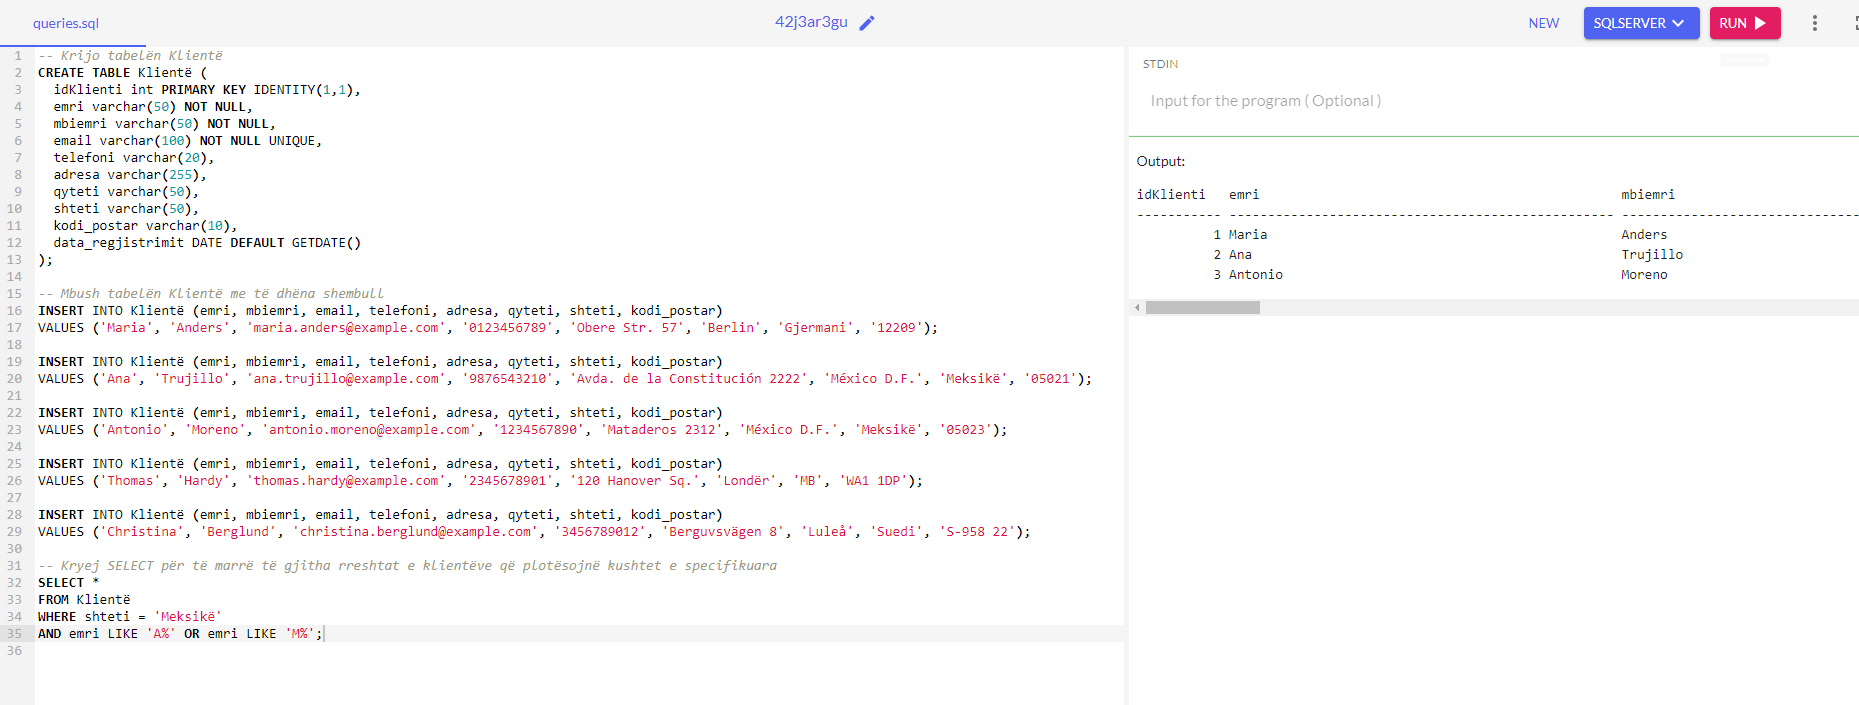
\includegraphics{./Figs/query17.png}
\end{frame}

\begin{frame}{Operatori OR}
\phantomsection\label{operatori-or}
\begin{itemize}
\item
  Klauzola WHERE mund të përmbajë një ose më shumë operatorë OR.
\item
  Operatori OR përdoret për të filtruar të dhënat bazuar në më shumë se
  një kusht, si p.sh. nëse dëshironi të ktheni të gjithë klientët nga
  Meksika, por edhe ata nga Spanja:
\end{itemize}
\end{frame}

\begin{frame}{Shembull}
\phantomsection\label{shembull-32}
Zgjidhni të gjithë klientët nga Meksika ose Spanja:
\end{frame}

\begin{frame}[fragile]{Shembull}
\phantomsection\label{shembull-33}
\AddToHookNext{env/Highlighting/begin}{\tiny}

\begin{Shaded}
\begin{Highlighting}[]
\CommentTok{{-}{-} Kryej SELECT për të marrë të gjitha rreshtat e klientëve që plotësojnë kushtet e specifikuara}
\KeywordTok{SELECT} \OperatorTok{*} 
\KeywordTok{FROM}\NormalTok{ Klientë}
\KeywordTok{WHERE}\NormalTok{ shteti }\OperatorTok{=} \StringTok{\textquotesingle{}Meksikë\textquotesingle{}} \KeywordTok{OR}\NormalTok{ shteti }\OperatorTok{=} \StringTok{\textquotesingle{}Spain\textquotesingle{}}
\end{Highlighting}
\end{Shaded}
\end{frame}

\begin{frame}{Shembull}
\phantomsection\label{shembull-34}
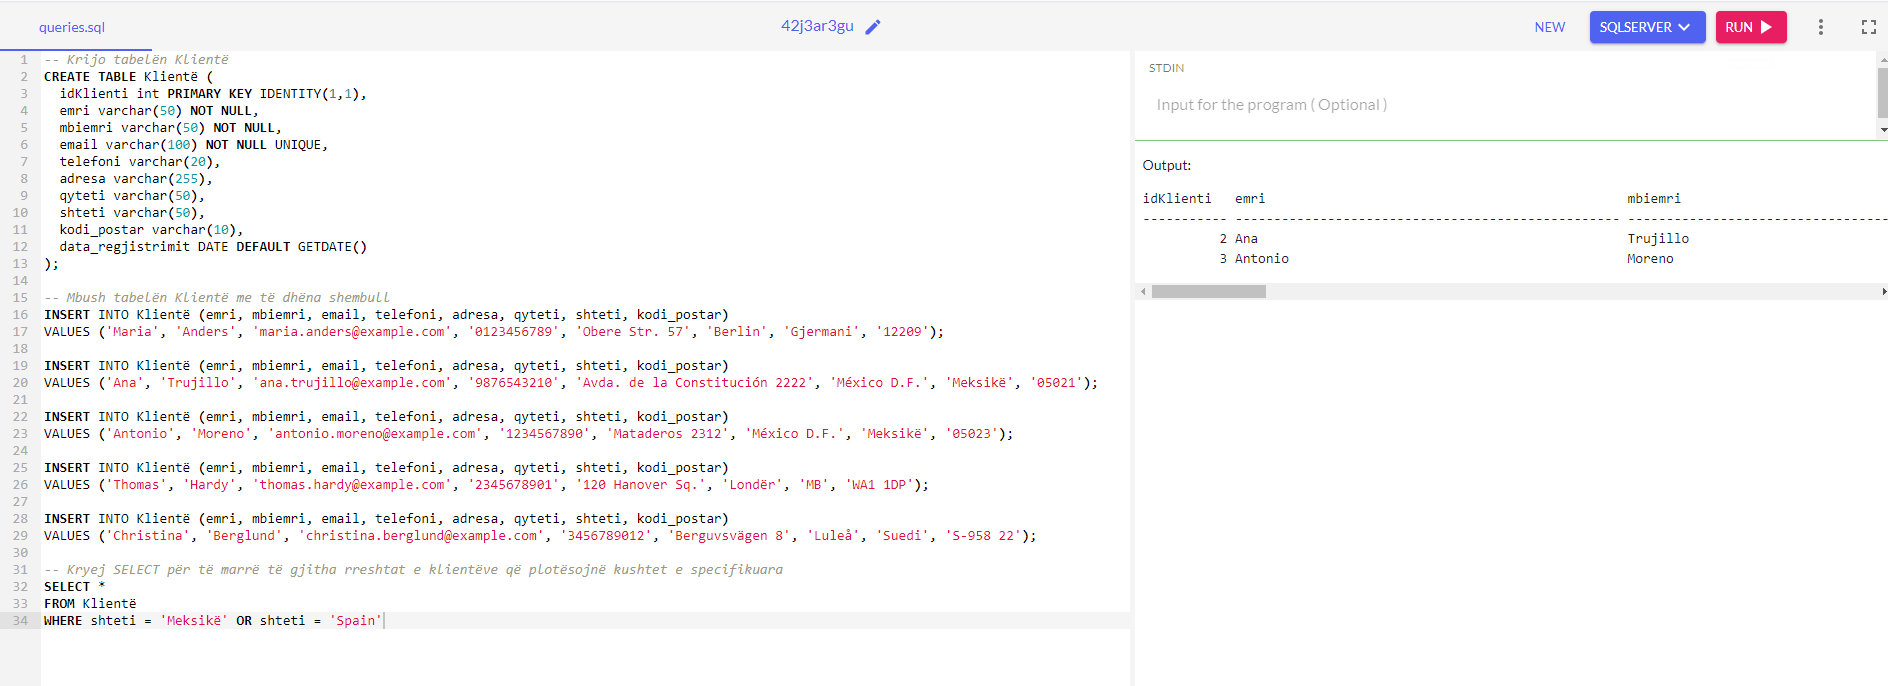
\includegraphics{./Figs/query18.png}
\end{frame}

\begin{frame}{Të paktën një kusht duhet të jetë i vërtetë}
\phantomsection\label{tuxeb-paktuxebn-njuxeb-kusht-duhet-tuxeb-jetuxeb-i-vuxebrtetuxeb}
\begin{itemize}
\item
  Deklarata e mëposhtme SQL zgjedh të gjitha fushat nga Klientë ku
  secili qytet është ``Berlin''
\item
  Emri i Klientit fillon me shkronjën ``G'' ose Vendi është
  ``Norvegji'':
\end{itemize}
\end{frame}

\begin{frame}[fragile]{Fillojmë me një tabelë}
\phantomsection\label{fillojmuxeb-me-njuxeb-tabeluxeb-8}
\AddToHookNext{env/Highlighting/begin}{\tiny}

\begin{Shaded}
\begin{Highlighting}[]
\CommentTok{{-}{-} Krijo tabelën Klientë}
\KeywordTok{CREATE} \KeywordTok{TABLE}\NormalTok{ Klientë (}
\NormalTok{  idKlienti }\DataTypeTok{int} \KeywordTok{PRIMARY} \KeywordTok{KEY}\NormalTok{ IDENTITY(}\DecValTok{1}\NormalTok{,}\DecValTok{1}\NormalTok{),}
\NormalTok{  emri }\DataTypeTok{varchar}\NormalTok{(}\DecValTok{50}\NormalTok{) }\KeywordTok{NOT} \KeywordTok{NULL}\NormalTok{,}
\NormalTok{  mbiemri }\DataTypeTok{varchar}\NormalTok{(}\DecValTok{50}\NormalTok{) }\KeywordTok{NOT} \KeywordTok{NULL}\NormalTok{,}
\NormalTok{  email }\DataTypeTok{varchar}\NormalTok{(}\DecValTok{100}\NormalTok{) }\KeywordTok{NOT} \KeywordTok{NULL} \KeywordTok{UNIQUE}\NormalTok{,}
\NormalTok{  telefoni }\DataTypeTok{varchar}\NormalTok{(}\DecValTok{20}\NormalTok{),}
\NormalTok{  adresa }\DataTypeTok{varchar}\NormalTok{(}\DecValTok{255}\NormalTok{),}
\NormalTok{  qyteti }\DataTypeTok{varchar}\NormalTok{(}\DecValTok{50}\NormalTok{),}
\NormalTok{  shteti }\DataTypeTok{varchar}\NormalTok{(}\DecValTok{50}\NormalTok{),}
\NormalTok{  kodi\_postar }\DataTypeTok{varchar}\NormalTok{(}\DecValTok{10}\NormalTok{),}
\NormalTok{  data\_regjistrimit }\DataTypeTok{DATE} \KeywordTok{DEFAULT}\NormalTok{ GETDATE()}
\NormalTok{);}
\end{Highlighting}
\end{Shaded}
\end{frame}

\begin{frame}[fragile]{Fillojmë me një tabelë}
\phantomsection\label{fillojmuxeb-me-njuxeb-tabeluxeb-9}
\AddToHookNext{env/Highlighting/begin}{\tiny}

\begin{Shaded}
\begin{Highlighting}[]
\CommentTok{{-}{-} Mbush tabelën Klientë me të dhëna shembull}
\KeywordTok{INSERT} \KeywordTok{INTO}\NormalTok{ Klientë (emri, mbiemri, email, telefoni, adresa, qyteti, shteti, kodi\_postar)}
\KeywordTok{VALUES}\NormalTok{ (}\StringTok{\textquotesingle{}Maria\textquotesingle{}}\NormalTok{, }\StringTok{\textquotesingle{}Anders\textquotesingle{}}\NormalTok{, }\StringTok{\textquotesingle{}maria.anders@example.com\textquotesingle{}}\NormalTok{, }\StringTok{\textquotesingle{}0123456789\textquotesingle{}}\NormalTok{, }\StringTok{\textquotesingle{}Obere Str. 57\textquotesingle{}}\NormalTok{, }\StringTok{\textquotesingle{}Berlin\textquotesingle{}}\NormalTok{, }\StringTok{\textquotesingle{}Gjermani\textquotesingle{}}\NormalTok{, }\StringTok{\textquotesingle{}12209\textquotesingle{}}\NormalTok{);}

\KeywordTok{INSERT} \KeywordTok{INTO}\NormalTok{ Klientë (emri, mbiemri, email, telefoni, adresa, qyteti, shteti, kodi\_postar)}
\KeywordTok{VALUES}\NormalTok{ (}\StringTok{\textquotesingle{}Ana\textquotesingle{}}\NormalTok{, }\StringTok{\textquotesingle{}Trujillo\textquotesingle{}}\NormalTok{, }\StringTok{\textquotesingle{}ana.trujillo@example.com\textquotesingle{}}\NormalTok{, }\StringTok{\textquotesingle{}9876543210\textquotesingle{}}\NormalTok{, }\StringTok{\textquotesingle{}Avda. de la Constitución 2222\textquotesingle{}}\NormalTok{, }\StringTok{\textquotesingle{}México D.F.\textquotesingle{}}\NormalTok{, }\StringTok{\textquotesingle{}Meksikë\textquotesingle{}}\NormalTok{, }\StringTok{\textquotesingle{}05021\textquotesingle{}}\NormalTok{);}

\KeywordTok{INSERT} \KeywordTok{INTO}\NormalTok{ Klientë (emri, mbiemri, email, telefoni, adresa, qyteti, shteti, kodi\_postar)}
\KeywordTok{VALUES}\NormalTok{ (}\StringTok{\textquotesingle{}Antonio\textquotesingle{}}\NormalTok{, }\StringTok{\textquotesingle{}Moreno\textquotesingle{}}\NormalTok{, }\StringTok{\textquotesingle{}antonio.moreno@example.com\textquotesingle{}}\NormalTok{, }\StringTok{\textquotesingle{}1234567890\textquotesingle{}}\NormalTok{, }\StringTok{\textquotesingle{}Mataderos 2312\textquotesingle{}}\NormalTok{, }\StringTok{\textquotesingle{}México D.F.\textquotesingle{}}\NormalTok{, }\StringTok{\textquotesingle{}Meksikë\textquotesingle{}}\NormalTok{, }\StringTok{\textquotesingle{}05023\textquotesingle{}}\NormalTok{);}

\KeywordTok{INSERT} \KeywordTok{INTO}\NormalTok{ Klientë (emri, mbiemri, email, telefoni, adresa, qyteti, shteti, kodi\_postar)}
\KeywordTok{VALUES}\NormalTok{ (}\StringTok{\textquotesingle{}Thomas\textquotesingle{}}\NormalTok{, }\StringTok{\textquotesingle{}Hardy\textquotesingle{}}\NormalTok{, }\StringTok{\textquotesingle{}thomas.hardy@example.com\textquotesingle{}}\NormalTok{, }\StringTok{\textquotesingle{}2345678901\textquotesingle{}}\NormalTok{, }\StringTok{\textquotesingle{}120 Hanover Sq.\textquotesingle{}}\NormalTok{, }\StringTok{\textquotesingle{}Londër\textquotesingle{}}\NormalTok{, }\StringTok{\textquotesingle{}MB\textquotesingle{}}\NormalTok{, }\StringTok{\textquotesingle{}WA1 1DP\textquotesingle{}}\NormalTok{);}

\KeywordTok{INSERT} \KeywordTok{INTO}\NormalTok{ Klientë (emri, mbiemri, email, telefoni, adresa, qyteti, shteti, kodi\_postar)}
\KeywordTok{VALUES}\NormalTok{ (}\StringTok{\textquotesingle{}Christina\textquotesingle{}}\NormalTok{, }\StringTok{\textquotesingle{}Berglund\textquotesingle{}}\NormalTok{, }\StringTok{\textquotesingle{}christina.berglund@example.com\textquotesingle{}}\NormalTok{, }\StringTok{\textquotesingle{}3456789012\textquotesingle{}}\NormalTok{, }\StringTok{\textquotesingle{}Berguvsvägen 8\textquotesingle{}}\NormalTok{, }\StringTok{\textquotesingle{}Luleå\textquotesingle{}}\NormalTok{, }\StringTok{\textquotesingle{}Suedi\textquotesingle{}}\NormalTok{, }\StringTok{\textquotesingle{}S{-}958 22\textquotesingle{}}\NormalTok{);}

\KeywordTok{INSERT} \KeywordTok{INTO}\NormalTok{ Klientë (emri, mbiemri, email, telefoni, adresa, qyteti, shteti, kodi\_postar)}
\KeywordTok{VALUES}\NormalTok{ (}\StringTok{\textquotesingle{}Gabriel\textquotesingle{}}\NormalTok{, }\StringTok{\textquotesingle{}Garcia\textquotesingle{}}\NormalTok{, }\StringTok{\textquotesingle{}gabriel.garcia@example.com\textquotesingle{}}\NormalTok{, }\StringTok{\textquotesingle{}0698765432\textquotesingle{}}\NormalTok{, }\StringTok{\textquotesingle{}Calle Mayor 5\textquotesingle{}}\NormalTok{, }\StringTok{\textquotesingle{}Madrid\textquotesingle{}}\NormalTok{, }\StringTok{\textquotesingle{}Spanjë\textquotesingle{}}\NormalTok{, }\StringTok{\textquotesingle{}28013\textquotesingle{}}\NormalTok{);}

\KeywordTok{INSERT} \KeywordTok{INTO}\NormalTok{ Klientë (emri, mbiemri, email, telefoni, adresa, qyteti, shteti, kodi\_postar)}
\KeywordTok{VALUES}\NormalTok{ (}\StringTok{\textquotesingle{}Gonzalo\textquotesingle{}}\NormalTok{, }\StringTok{\textquotesingle{}Perez\textquotesingle{}}\NormalTok{, }\StringTok{\textquotesingle{}gonzalo.perez@example.com\textquotesingle{}}\NormalTok{, }\StringTok{\textquotesingle{}0687654321\textquotesingle{}}\NormalTok{, }\StringTok{\textquotesingle{}Gran Via 12\textquotesingle{}}\NormalTok{, }\StringTok{\textquotesingle{}Barcelona\textquotesingle{}}\NormalTok{, }\StringTok{\textquotesingle{}Spanjë\textquotesingle{}}\NormalTok{, }\StringTok{\textquotesingle{}08010\textquotesingle{}}\NormalTok{);}

\KeywordTok{INSERT} \KeywordTok{INTO}\NormalTok{ Klientë (emri, mbiemri, email, telefoni, adresa, qyteti, shteti, kodi\_postar)}
\KeywordTok{VALUES}\NormalTok{ (}\StringTok{\textquotesingle{}Rita\textquotesingle{}}\NormalTok{, }\StringTok{\textquotesingle{}Sanchez\textquotesingle{}}\NormalTok{, }\StringTok{\textquotesingle{}rita.sanchez@example.com\textquotesingle{}}\NormalTok{, }\StringTok{\textquotesingle{}0571234567\textquotesingle{}}\NormalTok{, }\StringTok{\textquotesingle{}Avenida Diagonal 123\textquotesingle{}}\NormalTok{, }\StringTok{\textquotesingle{}Barcelona\textquotesingle{}}\NormalTok{, }\StringTok{\textquotesingle{}Spanjë\textquotesingle{}}\NormalTok{, }\StringTok{\textquotesingle{}08018\textquotesingle{}}\NormalTok{);}
\end{Highlighting}
\end{Shaded}
\end{frame}

\begin{frame}[fragile]{Shembull}
\phantomsection\label{shembull-35}
\begin{Shaded}
\begin{Highlighting}[]
\CommentTok{{-}{-} Kryej SELECT për të marrë të gjitha rreshtat e klientëve që plotësojnë kushtet e specifikuara}
\KeywordTok{SELECT} \OperatorTok{*} \KeywordTok{FROM}\NormalTok{ Klientë}
\KeywordTok{WHERE}\NormalTok{ qyteti }\OperatorTok{=} \StringTok{\textquotesingle{}Berlin\textquotesingle{}} \KeywordTok{OR}\NormalTok{ emri }\KeywordTok{LIKE} \StringTok{\textquotesingle{}G\%\textquotesingle{}} \KeywordTok{OR}\NormalTok{ shteti }\OperatorTok{=} \StringTok{\textquotesingle{}Norway\textquotesingle{}}\NormalTok{;}
\end{Highlighting}
\end{Shaded}
\end{frame}

\begin{frame}{Shembull}
\phantomsection\label{shembull-36}
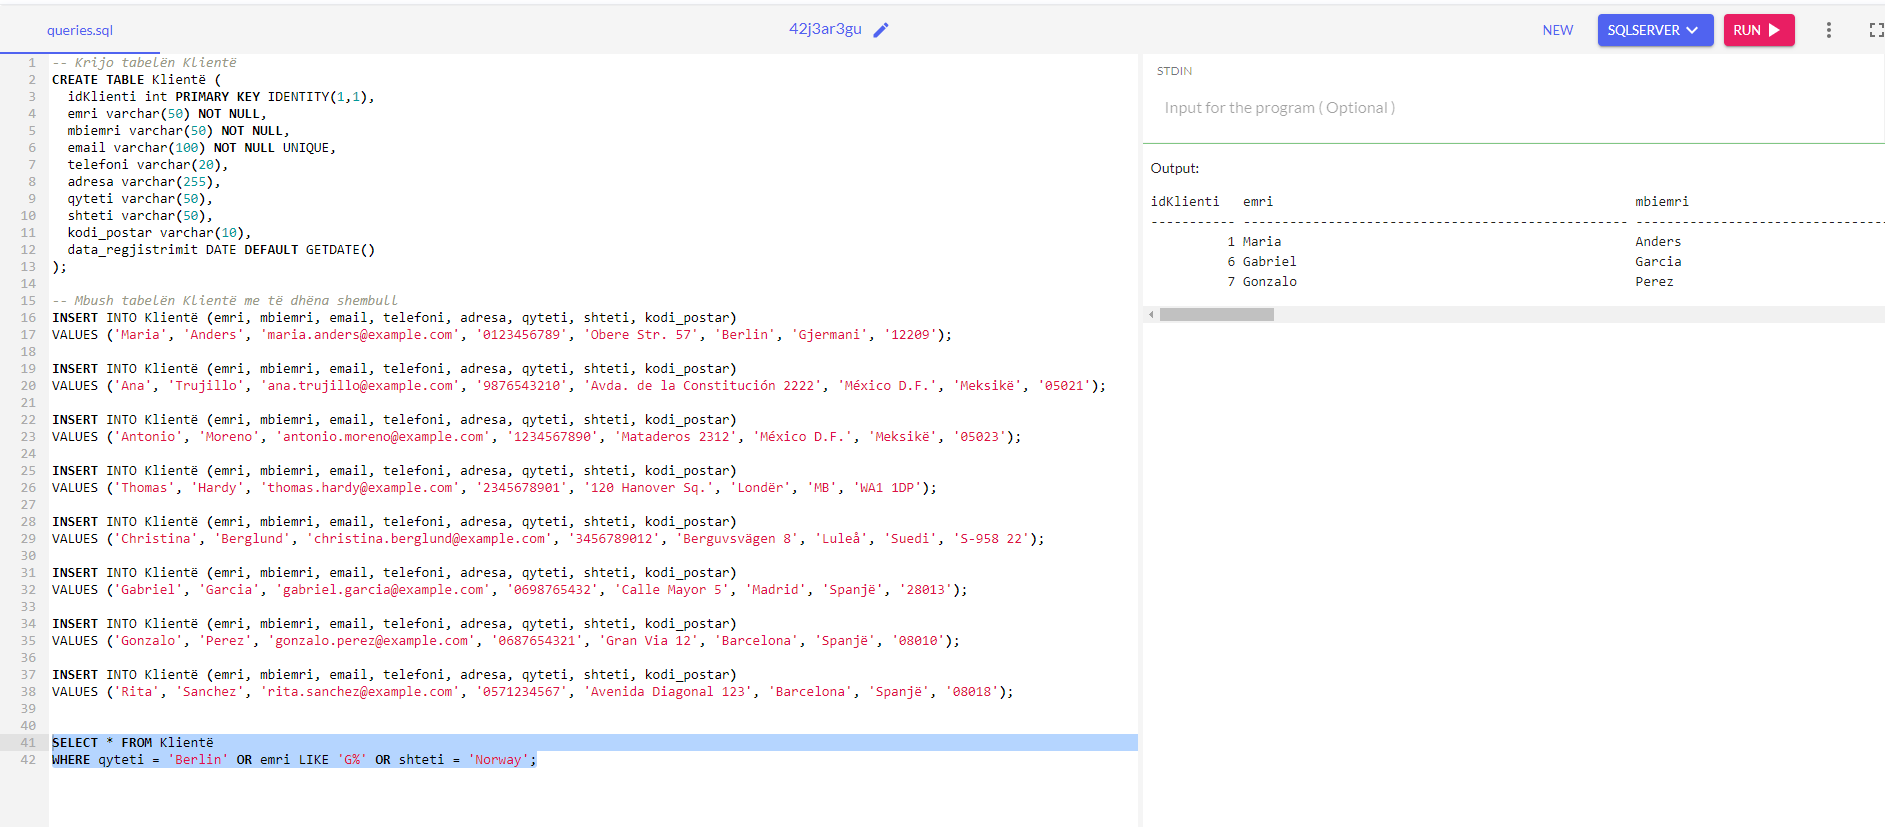
\includegraphics{./Figs/query19.png}
\end{frame}

\begin{frame}{Kombinimi AND dhe OR}
\phantomsection\label{kombinimi-and-dhe-or-2}
\begin{itemize}
\item
  Mund të kombinoni operatorët AND dhe OR.
\item
  Deklarata e mëposhtme SQL zgjedh të gjithë klientët nga Spanja që
  fillojnë me një ``G'' ose një ``R''.
\item
  Sigurohuni që të përdorni kllapa për të marrë rezultatin e saktë.
\end{itemize}
\end{frame}

\begin{frame}{Shembull}
\phantomsection\label{shembull-37}
Zgjidhni të gjithë klientët spanjollë që fillojnë me ``G'' ose ``R'':
\end{frame}

\begin{frame}[fragile]{Shembull}
\phantomsection\label{shembull-38}
\AddToHookNext{env/Highlighting/begin}{\tiny}

\begin{Shaded}
\begin{Highlighting}[]
\CommentTok{{-}{-} Kryej SELECT për të marrë të gjitha rreshtat e klientëve që plotësojnë kushtet e specifikuara}
\KeywordTok{SELECT} \OperatorTok{*} \KeywordTok{FROM}\NormalTok{ Klientë}
\KeywordTok{WHERE}\NormalTok{ shteti }\OperatorTok{=} \StringTok{\textquotesingle{}Spanjë\textquotesingle{}} \KeywordTok{AND}\NormalTok{ (emri }\KeywordTok{LIKE} \StringTok{\textquotesingle{}G\%\textquotesingle{}} \KeywordTok{OR}\NormalTok{ emri }\KeywordTok{LIKE} \StringTok{\textquotesingle{}R\%\textquotesingle{}}\NormalTok{);}
\end{Highlighting}
\end{Shaded}
\end{frame}

\begin{frame}{Shembull}
\phantomsection\label{shembull-39}
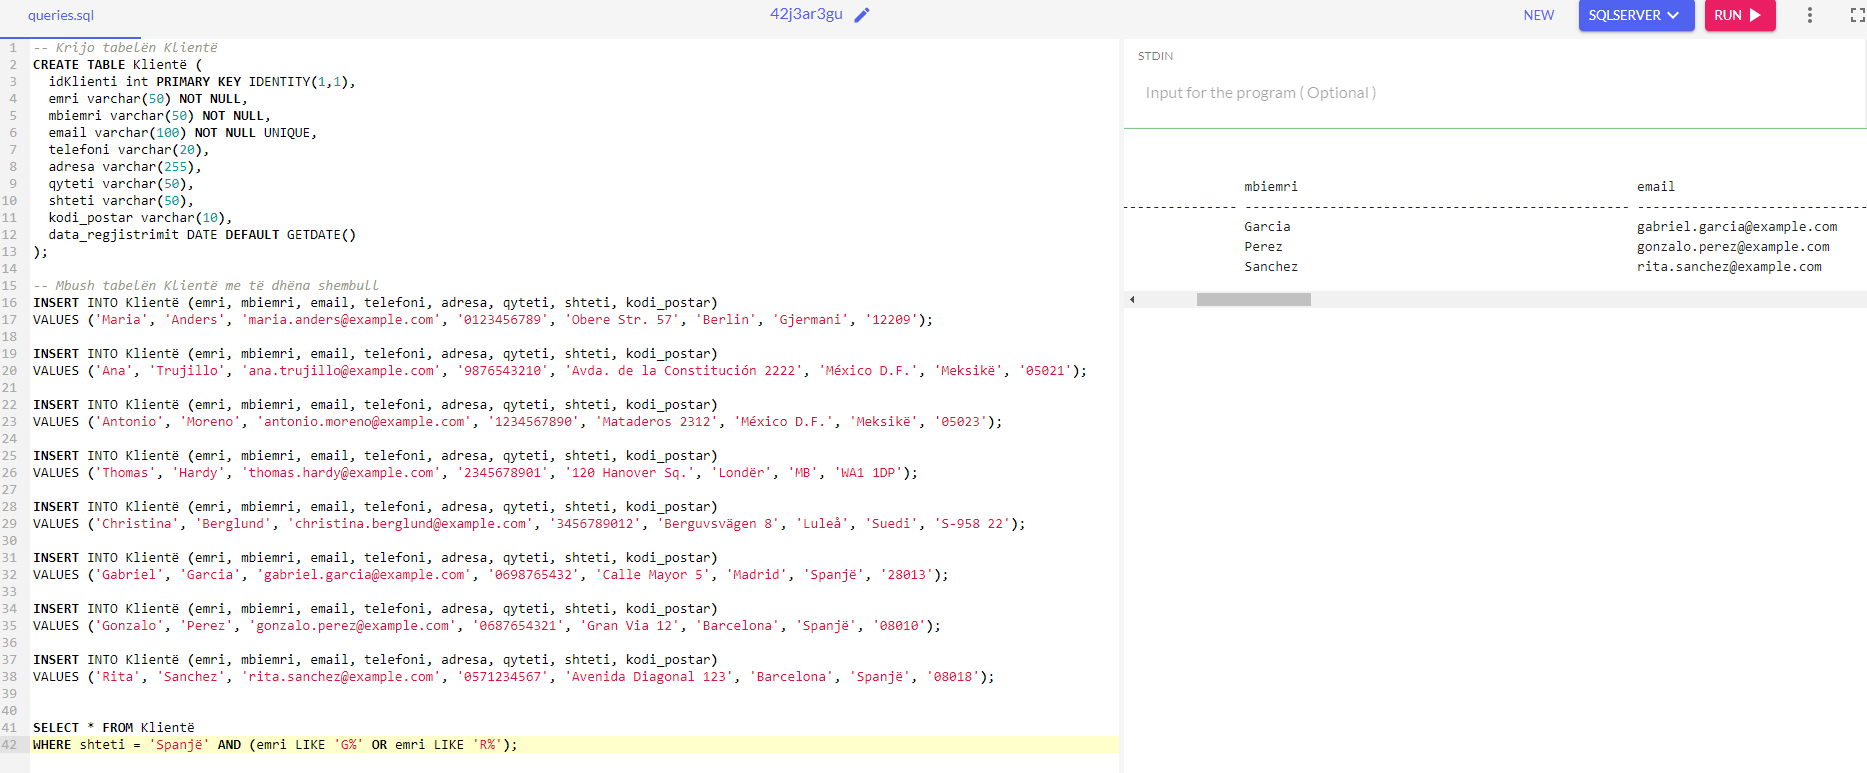
\includegraphics{./Figs/query20.png}
\end{frame}

\begin{frame}{Kombinimi AND dhe OR}
\phantomsection\label{kombinimi-and-dhe-or-3}
Pa kllapa, deklarata e përzgjedhur do t'i kthejë të gjithë klientët nga
Spanja që fillojnë me një ``G'', plus të gjithë klientët që fillojnë me
një ``R'', pavarësisht nga vlera e vendit:
\end{frame}

\begin{frame}{Shembull}
\phantomsection\label{shembull-40}
Zgjidhni të gjithë klientët që ose:

\begin{itemize}
\item
  janë nga Spanja dhe fillon ose me ``G'', ose
\item
  ju fillon me shkronjën ``R'':
\end{itemize}
\end{frame}

\begin{frame}[fragile]{Shembull}
\phantomsection\label{shembull-41}
\AddToHookNext{env/Highlighting/begin}{\tiny}

\begin{Shaded}
\begin{Highlighting}[]
\CommentTok{{-}{-} Kryej SELECT për të marrë të gjitha rreshtat e klientëve që plotësojnë kushtet e specifikuara}
\KeywordTok{SELECT} \OperatorTok{*} \KeywordTok{FROM}\NormalTok{ Klientë}
\KeywordTok{WHERE}\NormalTok{ shteti }\OperatorTok{=} \StringTok{\textquotesingle{}Spanjë\textquotesingle{}} \KeywordTok{AND}\NormalTok{ (emri }\KeywordTok{LIKE} \StringTok{\textquotesingle{}G\%\textquotesingle{}} \KeywordTok{OR}\NormalTok{ emri }\KeywordTok{LIKE} \StringTok{\textquotesingle{}R\%\textquotesingle{}}\NormalTok{);}
\end{Highlighting}
\end{Shaded}
\end{frame}

\begin{frame}{Shembull}
\phantomsection\label{shembull-42}
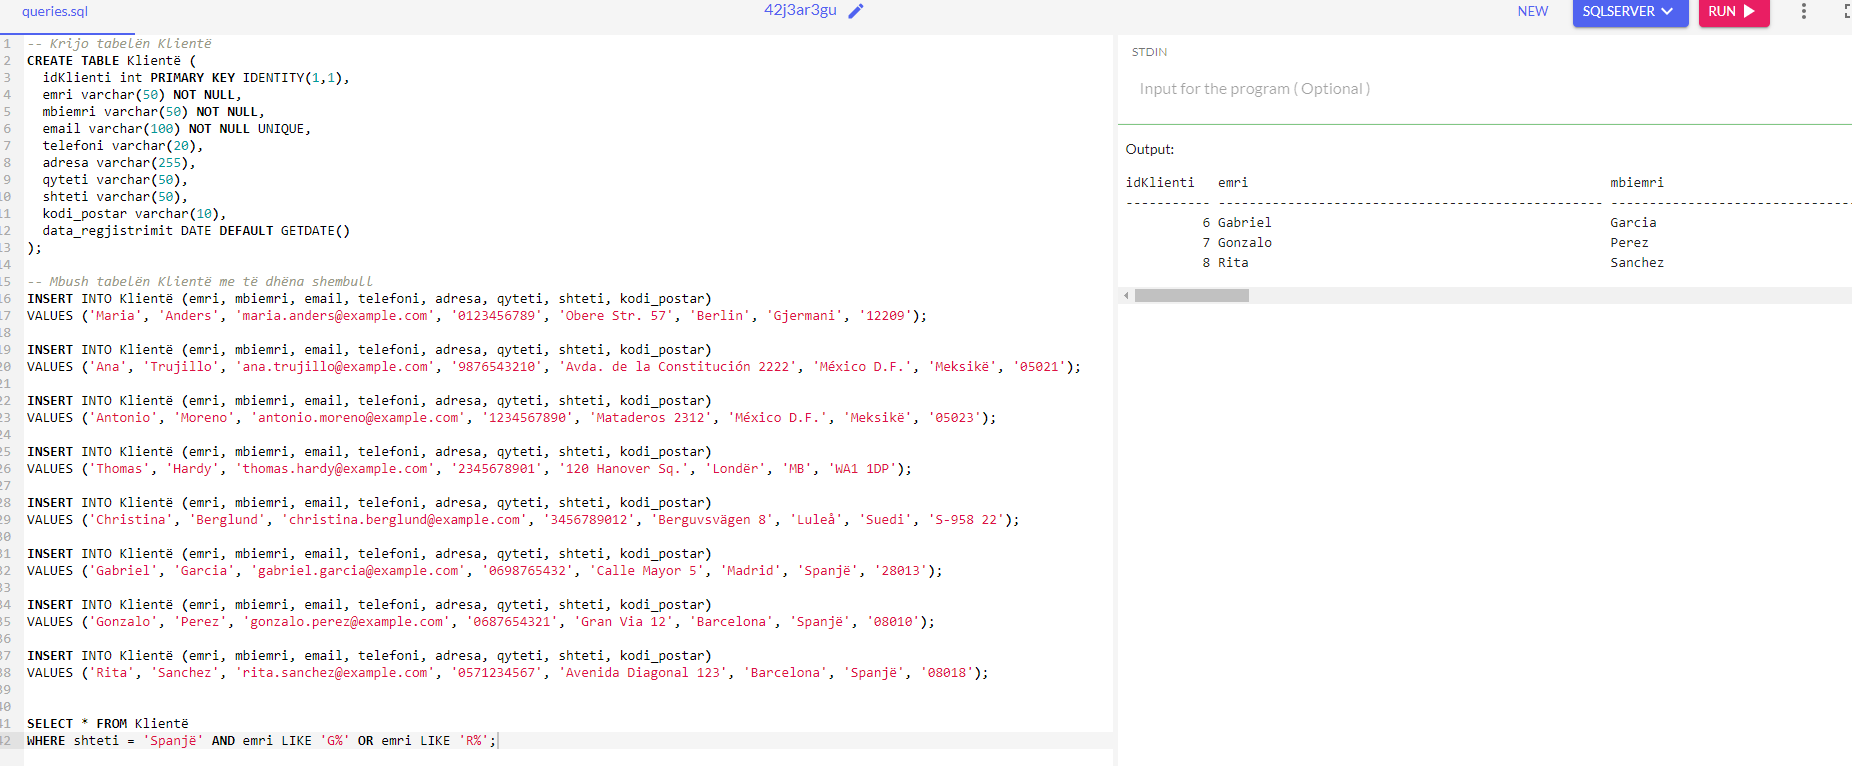
\includegraphics{./Figs/query21.png}
\end{frame}

\begin{frame}{Operatori NOT}
\phantomsection\label{operatori-not}
\begin{itemize}
\item
  Operatori NOT përdoret në kombinim me operatorë të tjerë për të dhënë
  rezultatin e kundërt, i quajtur edhe rezultat negativ.
\item
  Në deklaratën e përzgjedhur më poshtë duam të kthejmë të gjithë
  klientët që NUK janë nga Spanja:
\end{itemize}
\end{frame}

\begin{frame}{Shembull}
\phantomsection\label{shembull-43}
Zgjidhni vetëm klientët që NUK janë nga Spanja:
\end{frame}

\begin{frame}[fragile]{Shembull}
\phantomsection\label{shembull-44}
\AddToHookNext{env/Highlighting/begin}{\tiny}

\begin{Shaded}
\begin{Highlighting}[]
\CommentTok{{-}{-} Kryej SELECT për të marrë të gjitha rreshtat e klientëve që plotësojnë kushtet e specifikuara}
\KeywordTok{SELECT} \OperatorTok{*} \KeywordTok{FROM}\NormalTok{ Klientë}
\KeywordTok{WHERE} \KeywordTok{NOT}\NormalTok{ shteti }\OperatorTok{=} \StringTok{\textquotesingle{}Spanjë\textquotesingle{}}
\end{Highlighting}
\end{Shaded}
\end{frame}

\begin{frame}{Shembull}
\phantomsection\label{shembull-45}
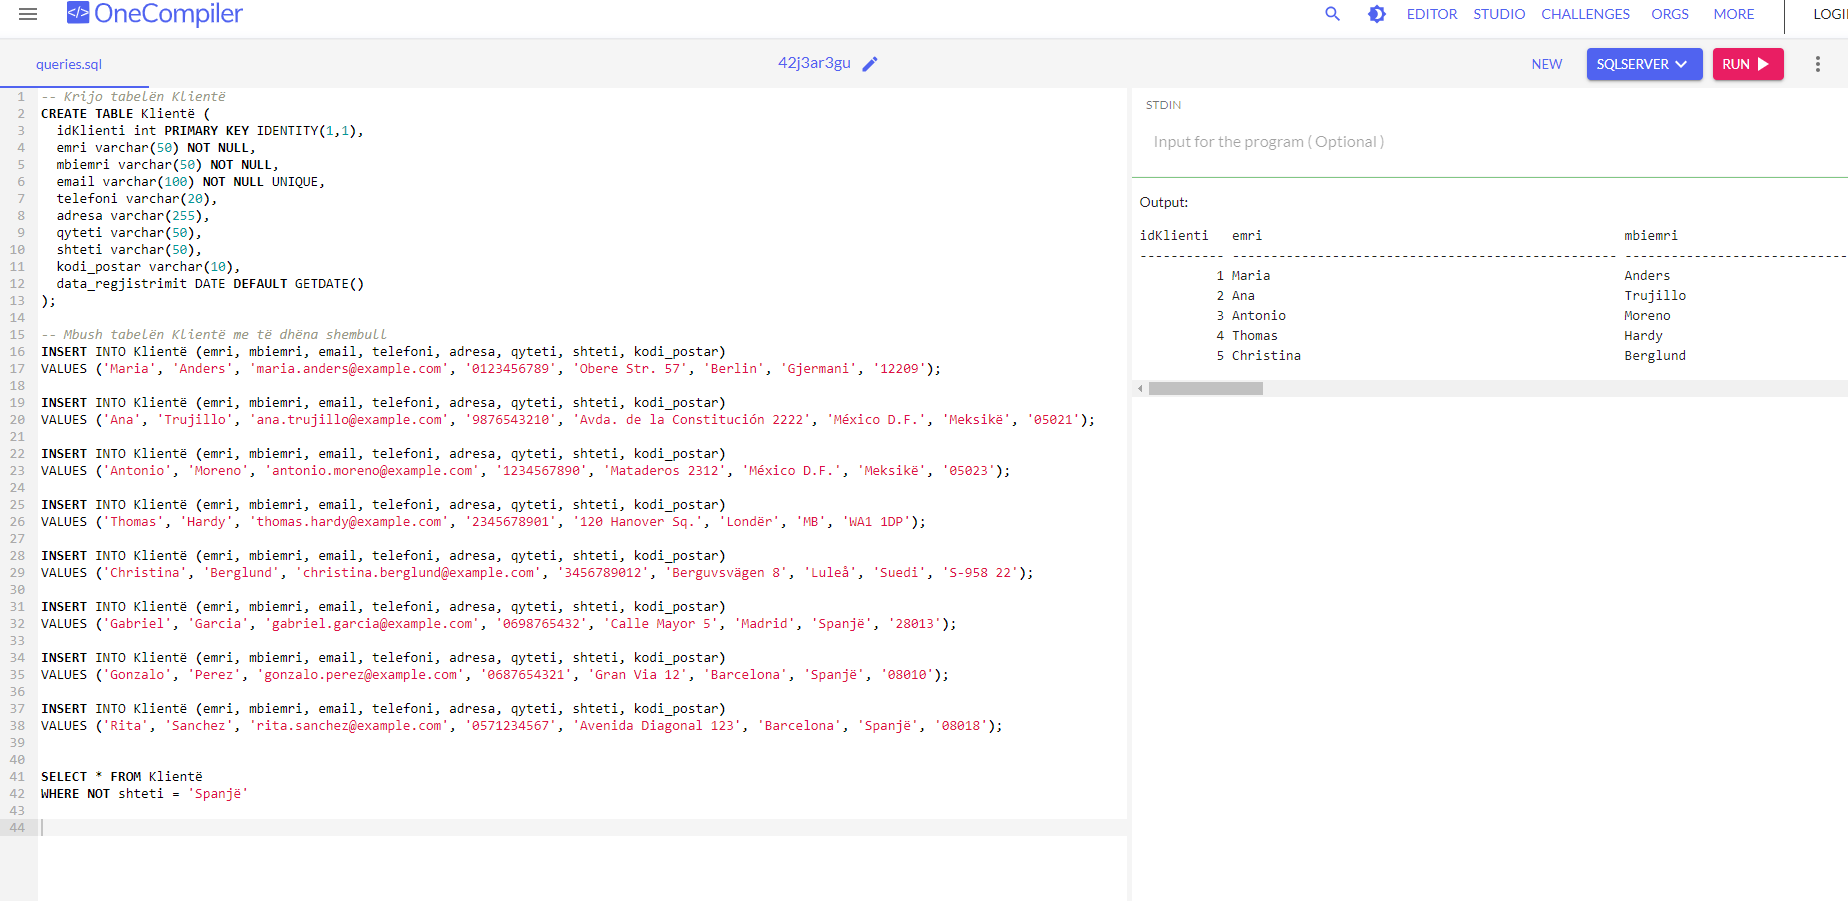
\includegraphics{./Figs/query22.png}
\end{frame}

\begin{frame}{NOT LIKE}
\phantomsection\label{not-like}
Zgjidhni klientët që nuk fillojnë me shkronjën ``A'':
\end{frame}

\begin{frame}[fragile]{NOT LIKE}
\phantomsection\label{not-like-1}
\AddToHookNext{env/Highlighting/begin}{\tiny}

\begin{Shaded}
\begin{Highlighting}[]
\CommentTok{{-}{-} Kryej SELECT për të marrë të gjitha rreshtat e klientëve që plotësojnë kushtet e specifikuara}
\KeywordTok{SELECT} \OperatorTok{*} \KeywordTok{FROM}\NormalTok{ Klientë}
\KeywordTok{WHERE}\NormalTok{ emri }\KeywordTok{NOT} \KeywordTok{LIKE} \StringTok{\textquotesingle{}A\%\textquotesingle{}}\NormalTok{;}
\end{Highlighting}
\end{Shaded}
\end{frame}

\begin{frame}{NOT LIKE}
\phantomsection\label{not-like-2}
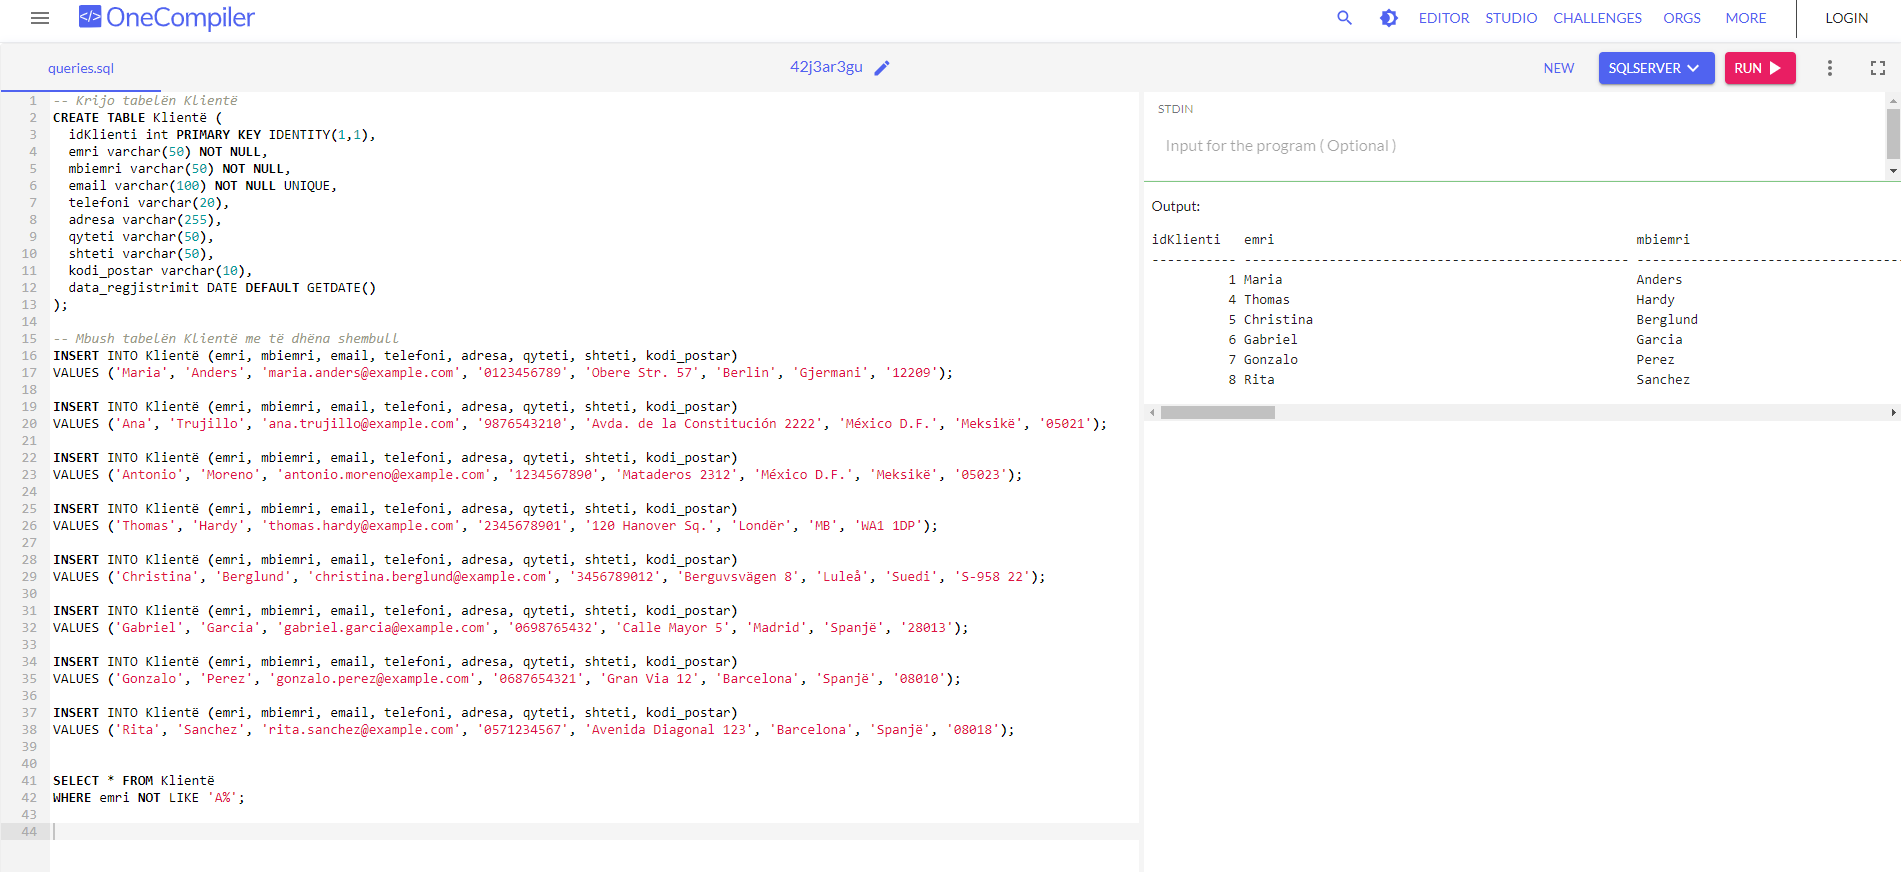
\includegraphics{./Figs/query23.png}
\end{frame}

\begin{frame}{NOT BETWEEN}
\phantomsection\label{not-between}
Zgjidhni klientët me një ID klienti jo midis 10 dhe 60:
\end{frame}

\begin{frame}[fragile]{NOT BETWEEN}
\phantomsection\label{not-between-1}
\AddToHookNext{env/Highlighting/begin}{\tiny}

\begin{Shaded}
\begin{Highlighting}[]
\CommentTok{{-}{-} Kryej SELECT për të marrë të gjitha rreshtat e klientëve që plotësojnë kushtet e specifikuara}

\KeywordTok{SELECT} \OperatorTok{*} \KeywordTok{FROM}\NormalTok{ Klientë}
\KeywordTok{WHERE}\NormalTok{ idKlienti }\KeywordTok{NOT} \KeywordTok{BETWEEN} \DecValTok{10} \KeywordTok{AND} \DecValTok{60}\NormalTok{;}
\end{Highlighting}
\end{Shaded}
\end{frame}

\begin{frame}{NOT BETWEEN}
\phantomsection\label{not-between-2}
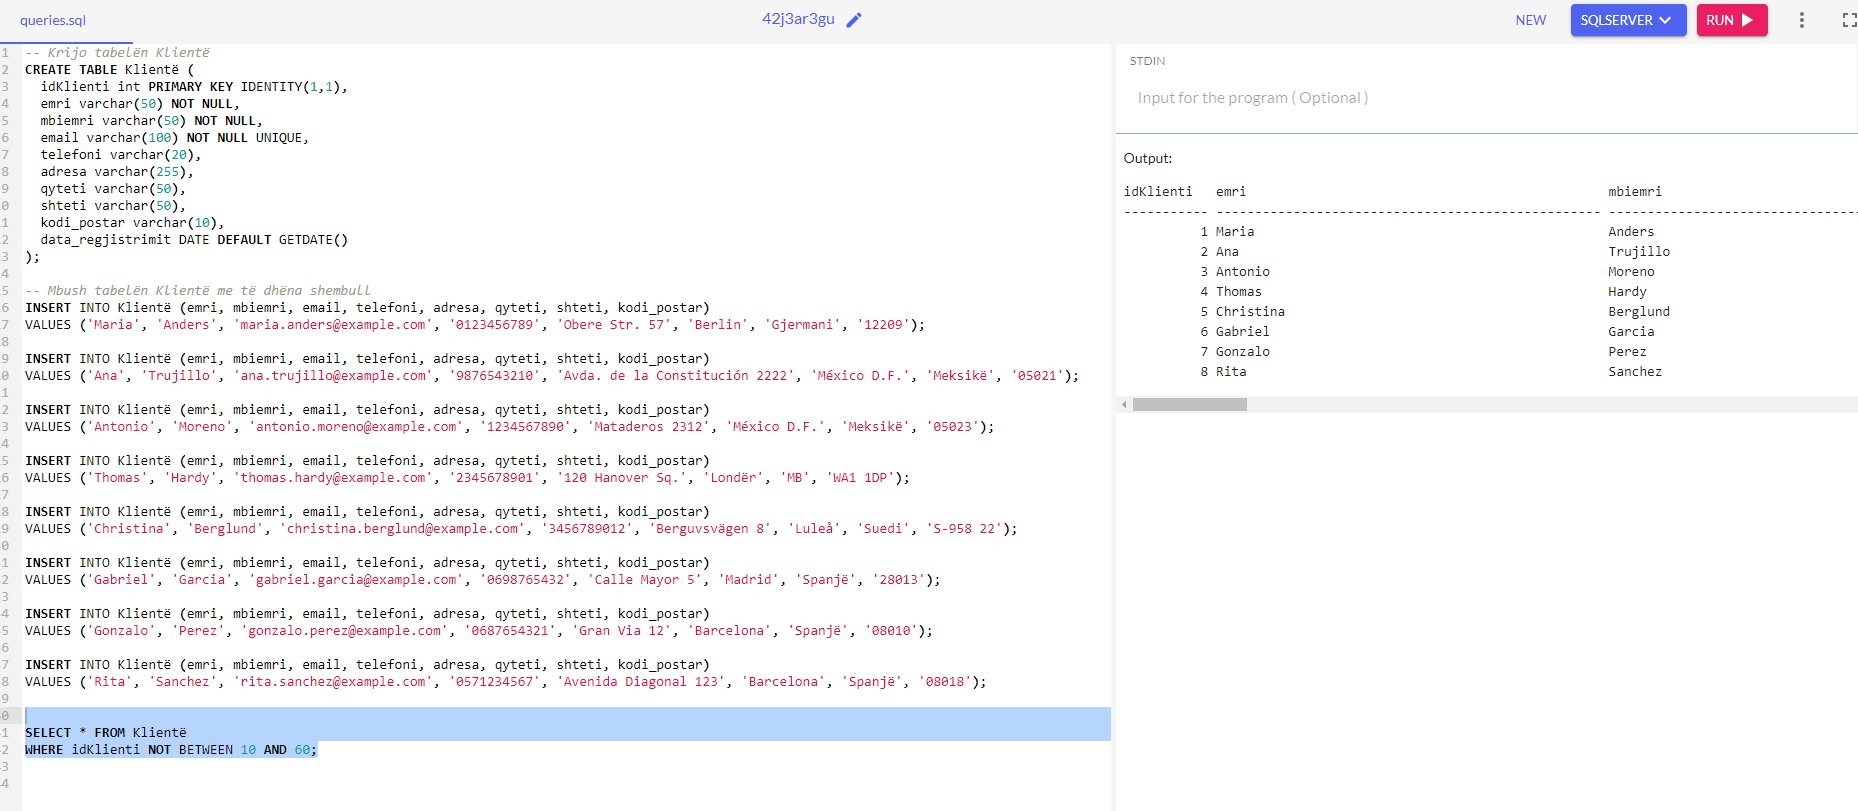
\includegraphics{./Figs/query24.png}
\end{frame}

\begin{frame}{NOT IN}
\phantomsection\label{not-in}
Zgjidhni klientët që nuk janë nga Parisi ose Londra:
\end{frame}

\begin{frame}[fragile]{NOT IN}
\phantomsection\label{not-in-1}
\AddToHookNext{env/Highlighting/begin}{\tiny}

\begin{Shaded}
\begin{Highlighting}[]
\CommentTok{{-}{-} Kryej SELECT për të marrë të gjitha rreshtat e klientëve që plotësojnë kushtet e specifikuara}

\KeywordTok{SELECT} \OperatorTok{*} \KeywordTok{FROM}\NormalTok{ Klientë}
\KeywordTok{WHERE}\NormalTok{ qyteti }\KeywordTok{NOT} \KeywordTok{IN}\NormalTok{ (}\StringTok{\textquotesingle{}Paris\textquotesingle{}}\NormalTok{, }\StringTok{\textquotesingle{}London\textquotesingle{}}\NormalTok{);}
\end{Highlighting}
\end{Shaded}
\end{frame}

\begin{frame}{NOT IN}
\phantomsection\label{not-in-2}
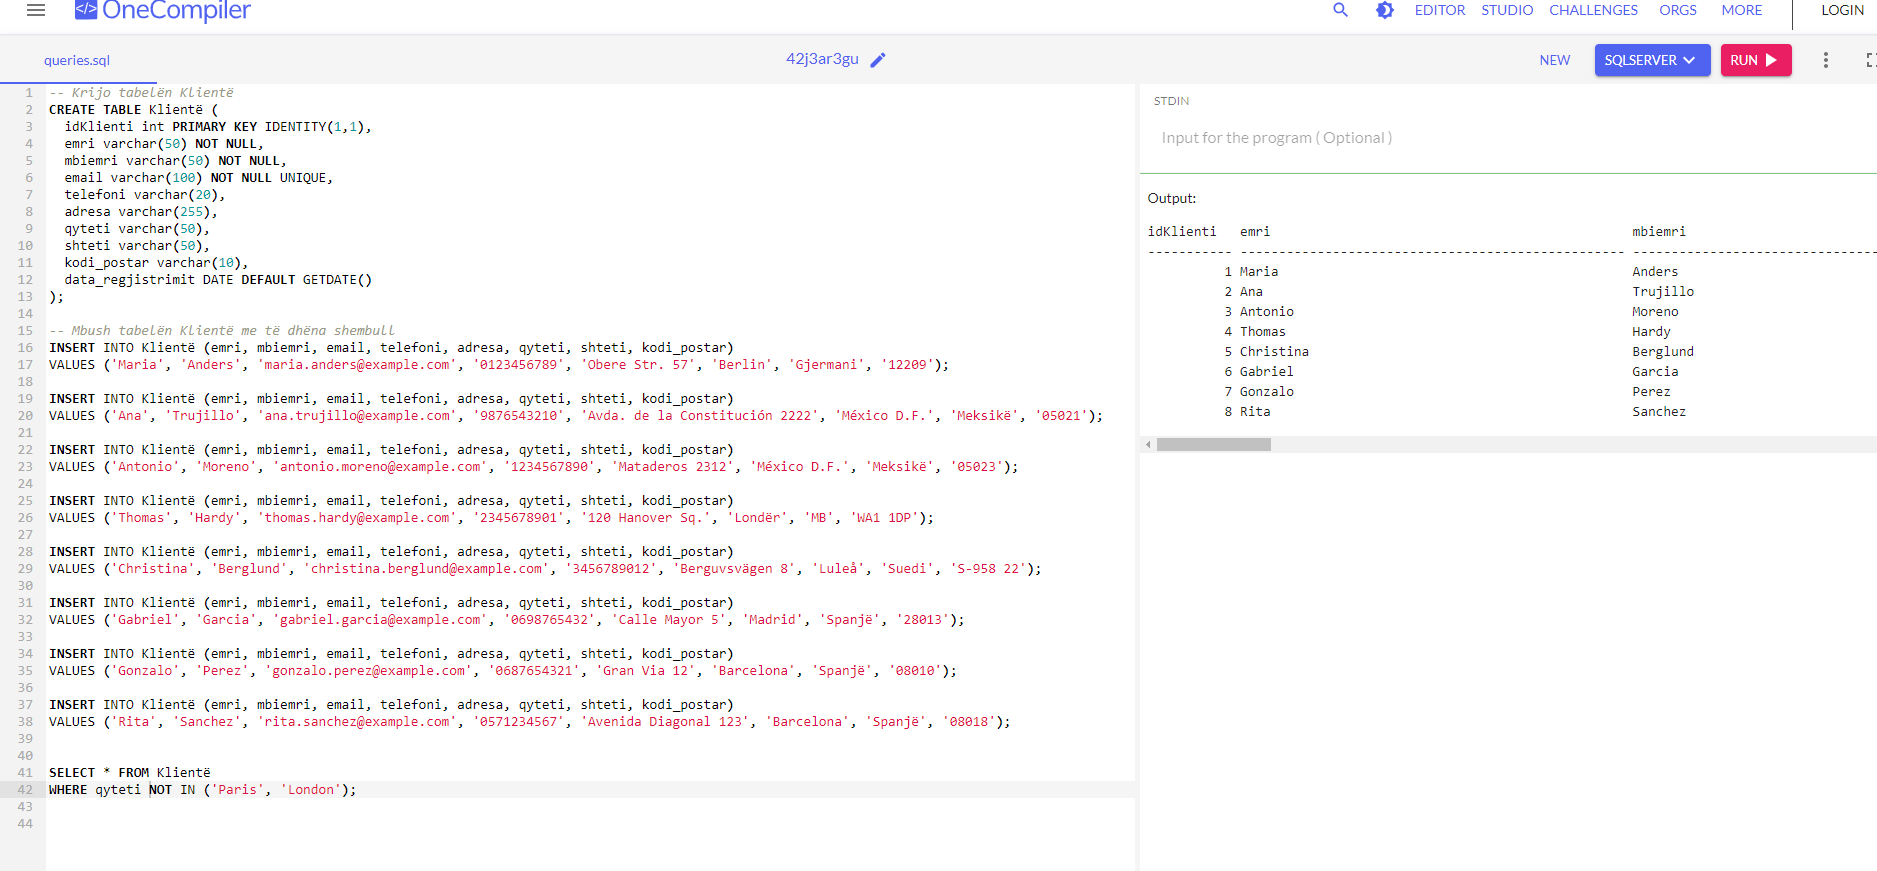
\includegraphics{./Figs/query26.png}
\end{frame}

\begin{frame}{NOT Greater Than}
\phantomsection\label{not-greater-than}
Zgjidhni klientët me një ID klienti jo më të madh se 50:
\end{frame}

\begin{frame}[fragile]{NOT Greater Than}
\phantomsection\label{not-greater-than-1}
\AddToHookNext{env/Highlighting/begin}{\tiny}

\begin{Shaded}
\begin{Highlighting}[]
\CommentTok{{-}{-} Kryej SELECT për të marrë të gjitha rreshtat e klientëve që plotësojnë kushtet e specifikuara}

\KeywordTok{SELECT} \OperatorTok{*} \KeywordTok{FROM}\NormalTok{ Klientë}
\KeywordTok{WHERE} \KeywordTok{NOT}\NormalTok{ idKlienti }\OperatorTok{\textgreater{}} \DecValTok{50}\NormalTok{;}
\end{Highlighting}
\end{Shaded}
\end{frame}

\begin{frame}{NOT Greater Than}
\phantomsection\label{not-greater-than-2}
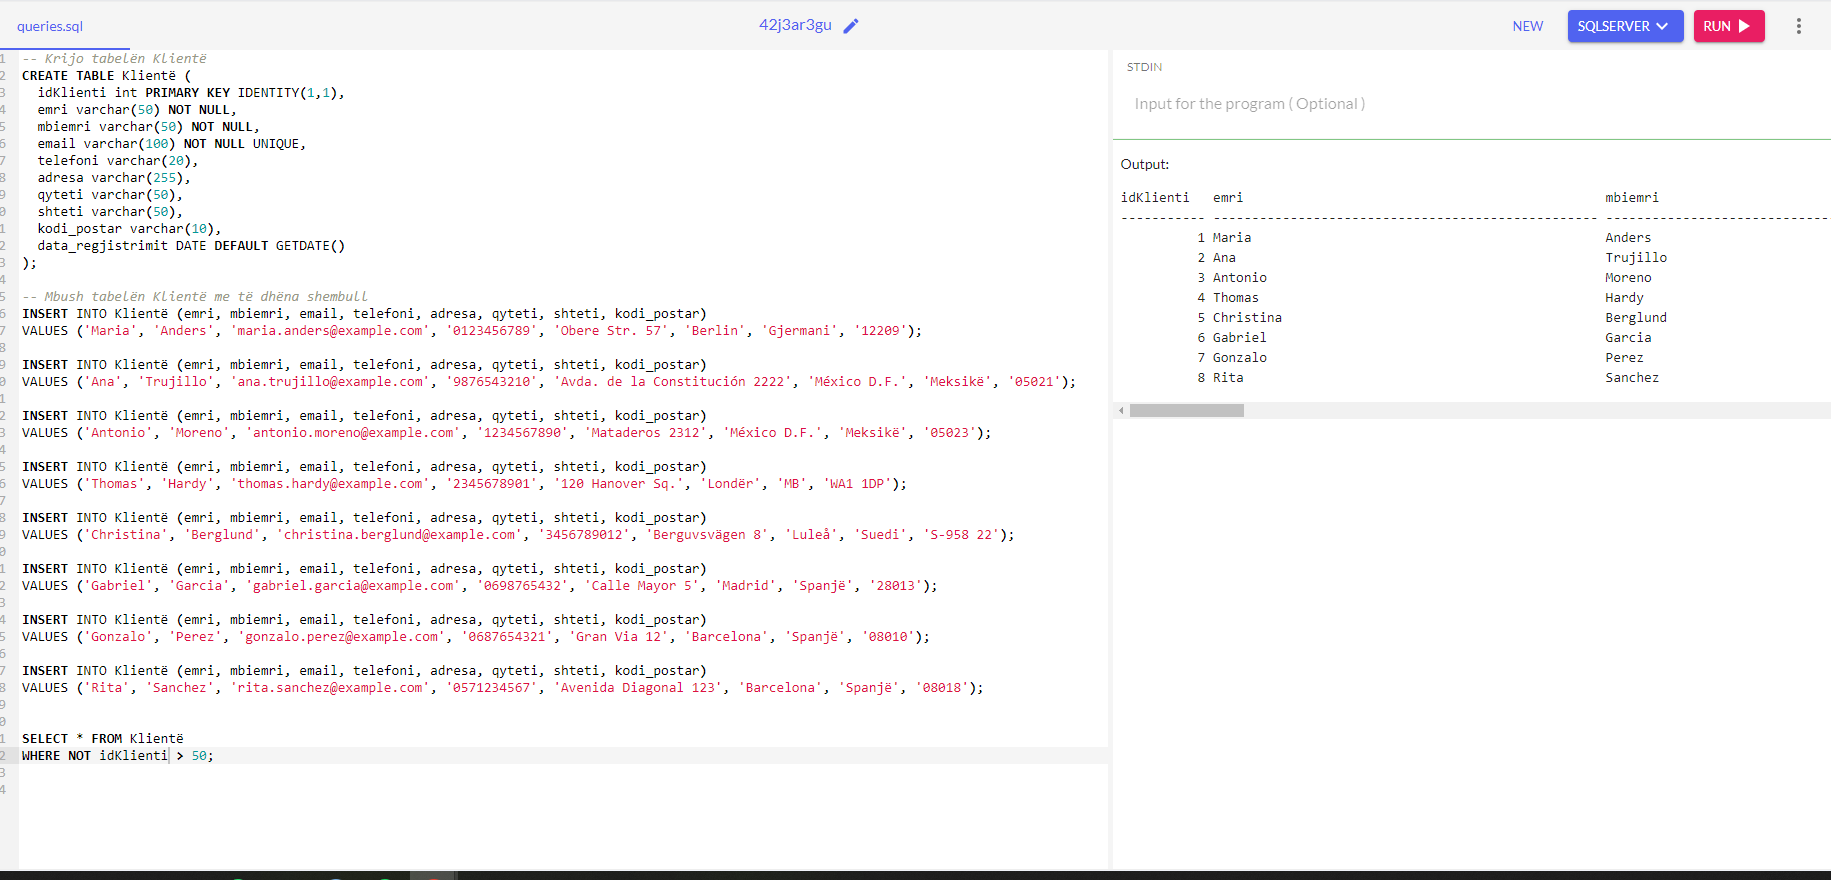
\includegraphics{./Figs/query27.png}

Shënim: Ekziston një operator jo më i madh se: !\textgreater{} që do
t'ju jepte të njëjtin rezultat.
\end{frame}

\begin{frame}{NOT Less Than}
\phantomsection\label{not-less-than}
Zgjidhni klientët me një ID klienti jo më pak se 50:
\end{frame}

\begin{frame}[fragile]{NOT Less Than}
\phantomsection\label{not-less-than-1}
\AddToHookNext{env/Highlighting/begin}{\tiny}

\begin{Shaded}
\begin{Highlighting}[]
\CommentTok{{-}{-} Kryej SELECT për të marrë të gjitha rreshtat e klientëve që plotësojnë kushtet e specifikuara}

\KeywordTok{SELECT} \OperatorTok{*} \KeywordTok{FROM}\NormalTok{ Klientë}
\KeywordTok{WHERE} \KeywordTok{NOT}\NormalTok{ idKlienti }\OperatorTok{\textless{}} \DecValTok{50}\NormalTok{;}
\end{Highlighting}
\end{Shaded}
\end{frame}

\begin{frame}{NOT Less Than}
\phantomsection\label{not-less-than-2}
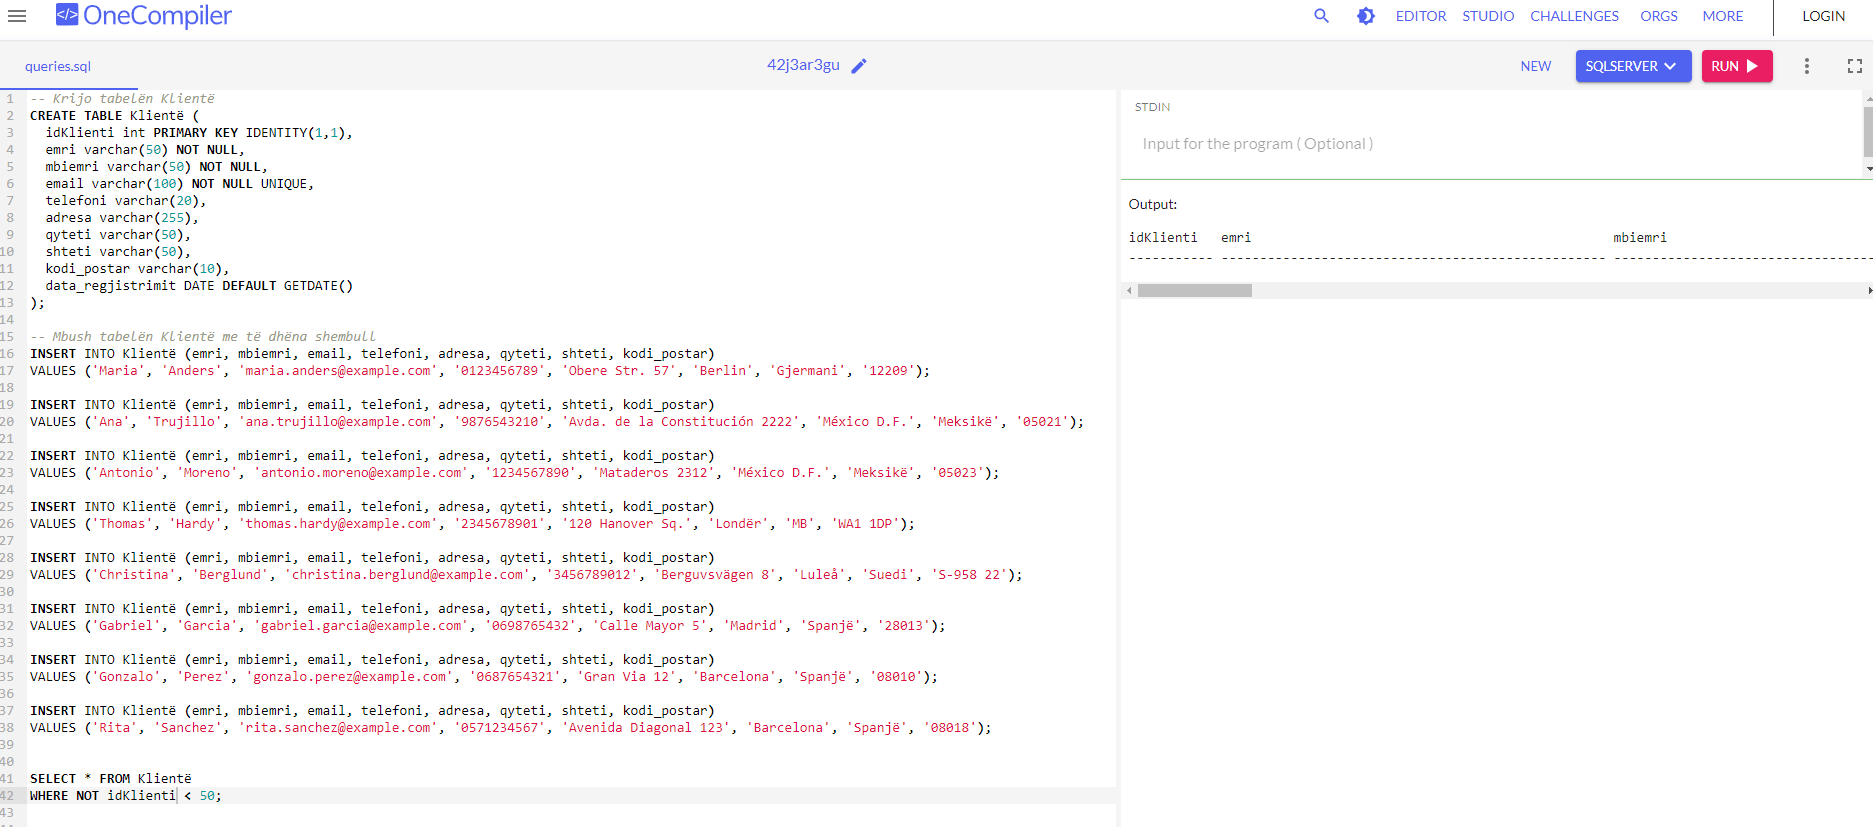
\includegraphics{./Figs/query29.png}
\end{frame}

\end{document}
